\documentclass[11pt,a4paper,oneside,openany]{report}

\usepackage[T1]{fontenc}
\usepackage[utf8]{inputenc}
\usepackage[english,french]{babel}
\usepackage{tgschola}
\usepackage[varg]{newtxmath}
\usepackage{microtype}

\usepackage[
  a4paper,
  left=25mm,
  right=20mm,
  top=20mm,
  bottom=20mm,
  headheight=16pt,
  headsep=7mm,
  footskip=10mm
]{geometry}
\usepackage{setspace}
\singlespacing
\setlength{\parindent}{1.5cm}
\setlength{\parskip}{0pt}
\setlength{\emergencystretch}{2em}

\usepackage{graphicx}
\graphicspath{{figures/}{../docs/}}
\usepackage{booktabs}
\usepackage{tabularx}
\usepackage{longtable}
\usepackage{array}
\usepackage{multirow}
\usepackage{makecell}
\usepackage{threeparttable}
\usepackage{float}
\usepackage{subcaption}
\usepackage{caption}
\captionsetup{font=small,labelfont=bf}

\usepackage[dvipsnames,table]{xcolor}
\definecolor{enstablue}{HTML}{143D59}
\definecolor{caimanblue}{HTML}{176B87}
\definecolor{caimangreen}{HTML}{3A7D44}
\definecolor{todoorange}{HTML}{B45309}

\usepackage{enumitem}
\setlist{nosep,leftmargin=*}
\usepackage{siunitx}
% Le préfixe micro doit rester droit : l'italique est réservé aux grandeurs.
\usepackage{upgreek}
\sisetup{locale=FR,per-mode=symbol,detect-all}
% Le préfixe micro doit rester droit (l'italique est réservé aux grandeurs) et
% ne pas introduire d'espace inter-unité : il est déclaré comme préfixe, non
% comme unité.
\DeclareSIPrefix{\micro}{\ensuremath{\upmu}}{-6}
\usepackage{amsmath}
\usepackage{csquotes}

\usepackage{listings}
\lstset{
  basicstyle=\ttfamily\small,
  frame=single,
  breaklines=true,
  columns=fullflexible,
  showstringspaces=false,
  keywordstyle=\color{caimanblue}\bfseries,
  commentstyle=\color{caimangreen}
}

\usepackage{tikz}
\usetikzlibrary{arrows.meta,positioning,shapes.geometric,fit}
\usepackage{pgfgantt}

\usepackage{titlesec}
\titleformat{\chapter}[display]
  {\normalfont\bfseries\color{enstablue}}
  {\fontsize{18}{20}\selectfont\chaptername\ \thechapter}
  {0.5ex}
  {\fontsize{22}{25}\selectfont}
\titleformat{\section}
  {\normalfont\fontsize{14}{17}\selectfont\bfseries\color{enstablue}}
  {\thesection}{0.7em}{}
\titleformat{\subsection}
  {\normalfont\fontsize{12}{15}\selectfont\bfseries\itshape}
  {\thesubsection}{0.7em}{}

\usepackage{fancyhdr}
\usepackage{emptypage}

\usepackage[
  backend=bibtex,
  style=numeric-comp,
  sorting=nyt,
  maxbibnames=8
]{biblatex}

\usepackage{hyperref}
\hypersetup{
  colorlinks=true,
  linkcolor=enstablue,
  citecolor=caimangreen,
  urlcolor=caimanblue,
  pdftitle={Rapport de PRe - Caiman},
  pdfauthor={Joab da Silva Bezerra},
  pdfsubject={Électronique embarquée et robotique sous-marine}
}
\usepackage[nameinlink,noabbrev]{cleveref}

\newcommand{\TODOJOAB}[1]{%
  \textcolor{todoorange}{\textbf{TODO\_JOAB :} #1}%
}

\newcommand{\GitCommit}[1]{\texttt{#1}}
\newcommand{\RepositoryPath}[1]{\texttt{#1}}

\newcommand{\EvidenceStatus}[1]{%
  \begingroup
  \setlength{\fboxsep}{2pt}%
  \colorbox{enstablue!10}{\textcolor{enstablue}{\textbf{#1}}}%
  \endgroup
}

\newcommand{\LogoOrPlaceholder}[3][32mm]{%
  \IfFileExists{#2}{%
    \includegraphics[width=#1]{#2}%
  }{%
    \fbox{\parbox[c][18mm][c]{\dimexpr#1-2\fboxsep-2\fboxrule\relax}{\centering\footnotesize #3}}%
  }%
}

\pagestyle{fancy}
\fancyhf{}
\fancyhead[LE]{\small\nouppercase{\leftmark}}
\fancyhead[RO]{\small\nouppercase{\rightmark}}
\fancyfoot[LE,RO]{\thepage}
\fancyfoot[LO,RE]{\small\StudentName\ -- \HostShortName\ -- \ConfidentialityShort}
\renewcommand{\headrulewidth}{0.4pt}
\renewcommand{\footrulewidth}{0.2pt}

\fancypagestyle{plain}{%
  \fancyhf{}
  \fancyfoot[LE,RO]{\thepage}
  \fancyfoot[LO,RE]{\small\StudentName\ -- \HostShortName\ -- \ConfidentialityShort}
  \renewcommand{\headrulewidth}{0pt}
  \renewcommand{\footrulewidth}{0.2pt}
}

\crefname{figure}{figure}{figures}
\crefname{table}{tableau}{tableaux}
\crefname{chapter}{chapitre}{chapitres}
\crefname{section}{section}{sections}
\crefname{equation}{équation}{équations}
\Crefname{equation}{Équation}{Équations}
\crefname{appendix}{annexe}{annexes}
\Crefname{appendix}{Annexe}{Annexes}
\crefname{lstlisting}{listing}{listings}
\Crefname{lstlisting}{Listing}{Listings}

\newcommand{\StudentName}{Joab da Silva Bezerra}
\newcommand{\ProgramName}{Diplôme d'ingénieur de l'ENSTA -- 2\textsuperscript{e} année -- spécialité Robotique autonome -- promotion 2027}
\newcommand{\AcademicYear}{2025--2026}

\newcommand{\ReportTitle}{Conception d'un essaim de robots subsurface}
\newcommand{\ReportSubtitle}{Électronique embarquée, simulation et prototypage d'une flotte de robots Caiman}
% Titre en anglais, exigé sur la page de résumé par les instructions de dépôt.
\newcommand{\ReportTitleEN}{Design of a subsurface robot swarm}
\newcommand{\ReportSubtitleEN}{Embedded electronics, simulation and prototyping of a Caiman robot fleet}

\newcommand{\HostName}{CNRS -- Lab-STICC (UMR 6285), campus ENSTA de Brest}
\newcommand{\HostShortName}{CNRS / Lab-STICC / ENSTA}
\newcommand{\HostTeam}{équipe ROBEX}
\newcommand{\HostAddress}{2, rue François Verny -- Brest}

\newcommand{\SupervisorOne}{Franck Ruffier}
\newcommand{\SupervisorOneRole}{Directeur de recherche CNRS en robotique, ROBEX / Lab-STICC}
\newcommand{\SupervisorTwo}{Quentin Brateau}
\newcommand{\SupervisorTwoRole}{Doctorant en robotique marine, accompagnement technique quotidien}
\newcommand{\AcademicTutor}{Philippe Xu}
\newcommand{\AcademicTutorRole}{Enseignant-chercheur, référent pédagogique ENSTA}

\newcommand{\StageStart}{1\textsuperscript{er} juin 2026}
\newcommand{\StageEnd}{31 août 2026}
\newcommand{\DefenseDate}{24 août 2026}
\newcommand{\Confidentiality}{Rapport de Projet de Recherche (PRe)}
\newcommand{\ConfidentialityShort}{Rapport de PRe}


\addbibresource{bibliography/references.bib}

\begin{document}

% Pagination continue à partir de la page de titre ; affichage à partir du résumé.
\pagenumbering{arabic}

\newgeometry{margin=20mm}
\begin{titlepage}
  \thispagestyle{empty}

  \noindent\begin{minipage}[t]{0.48\textwidth}
    \raggedright
    \LogoOrPlaceholder[72mm]{figures/logos/ensta_ip_paris_horizontal_bleu.png}{Logo ENSTA}
  \end{minipage}
  \hfill
  \begin{minipage}[t]{0.48\textwidth}
    \raggedleft
    \begingroup
      \setlength{\fboxsep}{2.5mm}%
      \colorbox{enstablue}{
\includegraphics[width=43mm]{figures/logos/labsticc_logo_officiel.png}}%
    \endgroup
  \end{minipage}

  \vspace{9mm}

  \begin{center}
    {\Large\bfseries Projet de Recherche (PRe)\par}
    \vspace{4mm}
    {\large \ProgramName\par}
    {\large Année universitaire \AcademicYear\par}

    \vspace{11mm}
    {\color{enstablue}\rule{0.9\textwidth}{1.2pt}\par}
    \vspace{7mm}
    {\fontsize{22}{27}\selectfont\bfseries\ReportTitle\par}
    \vspace{5mm}
    {\Large\itshape\ReportSubtitle\par}
    \vspace{7mm}
    {\color{enstablue}\rule{0.9\textwidth}{1.2pt}\par}

    \vspace{6mm}
    \includegraphics[width=0.50\textwidth,height=42mm,keepaspectratio]%
      {fabrication/cad_caiman_full_assembly.png}

    \vfill

    \begin{tabularx}{0.92\textwidth}{@{}>{\bfseries}l X@{}}
      Auteur : & \StudentName \\
      Organisme d'accueil : & \HostName, \HostTeam \\
      Tuteur principal : & \SupervisorOne{} -- \SupervisorOneRole \\
      Accompagnement technique : & \SupervisorTwo{} -- \SupervisorTwoRole \\
      Référent pédagogique : & \AcademicTutor{} -- \AcademicTutorRole \\
      Période : & du \StageStart{} au \StageEnd \\
      Soutenance : & \DefenseDate \\
    \end{tabularx}

    \vfill

    {\HostAddress\par}
    \vspace{4mm}
    {\bfseries\Confidentiality\par}
    \vspace{2mm}
    {\Large\bfseries\color{red}NON CONFIDENTIEL\par}
  \end{center}
\end{titlepage}
\restoregeometry

\setcounter{page}{2}

% Page de garde vierge (exigée par le guide de rédaction du PRe)
\thispagestyle{empty}
\null
\clearpage

\clearpage
\thispagestyle{empty}

\begin{center}
  \vspace*{20mm}
  {\Huge\bfseries Note de non-confidentialité\par}
  \vspace{15mm}
  {\color{enstablue}\rule{0.8\textwidth}{1.5pt}\par}
\end{center}

\vspace{15mm}

\noindent Le présent rapport de stage de Projet de Recherche (PRe), intitulé :

\begin{center}
  \vspace{6mm}
  {\Large\bfseries\color{enstablue} \ReportTitle\par}
  \vspace{4mm}
  {\large\itshape \ReportSubtitle\par}
  \vspace{6mm}
\end{center}

\noindent effectué par \StudentName{} du \StageStart{} au \StageEnd{} au sein du \HostName, unité \HostTeam, est classé \textbf{non confidentiel}.

\vspace{10mm}

\noindent Le document sera archivé au format électronique par la bibliothèque de l'ENSTA Paris.

\vspace{10mm}

\noindent La convention de stage conclue avec le CNRS soumet toutefois les publications et communications relatives au contenu du stage à une autorisation préalable de l'organisme d'accueil. Les conditions de mise en ligne du présent rapport sont donc celles précisées par l'organisme sur l'attestation de confidentialité / non-confidentialité qui l'accompagne.

\vspace{25mm}

\noindent\begin{minipage}[t]{0.45\textwidth}
  \textbf{L'élève stagiaire}\\[10mm]
  \StudentName
\end{minipage}
\hfill
\begin{minipage}[t]{0.45\textwidth}
  \textbf{Le tuteur d'accueil}\\[10mm]
  \SupervisorOne{} \\ \SupervisorOneRole
\end{minipage}

\clearpage


\begingroup
\pagestyle{empty}
\chapter*{Remerciements}
\addcontentsline{toc}{chapter}{Remerciements}

Je remercie Franck Ruffier, directeur de recherche CNRS au Lab-STICC et tuteur de ce projet, pour son accueil dans l'équipe ROBEX et pour la liberté qu'il m'a laissée dans la conduite du travail.

Je remercie Philippe Xu, enseignant-chercheur à l'ENSTA Paris et référent pédagogique de ce PRe, pour son suivi tout au long du stage.

Je remercie enfin Quentin Brateau, doctorant en robotique marine, pour l'accompagnement technique quotidien sur le projet Caiman, ainsi que l'ensemble de l'équipe du Lab-STICC sur le campus ENSTA de Brest pour la qualité des échanges.

\clearpage

\endgroup

\clearpage
\phantomsection
\addcontentsline{toc}{chapter}{Résumé et abstract}

\section*{Résumé}

Ce rapport présente la conception et la préparation à la fabrication d'une carte électronique embarquée destinée à une flotte de robots sous-marins autonomes. Le travail couvre la correction du schéma, la reprise du routage, la génération des fichiers de production et une première architecture logicielle. Un essai exploratoire STM32/centrale inertielle a précédé le développement d'un simulateur déterministe de mission bathymétrique : cinq AUV, communication radio limitée aux contacts de surface, supervision, trames sécurisées de 32 octets, défauts et scénario de capture. Son interface Web a été conteneurisée et déployée sur une VPS. Un prototype HIL fondé sur un ESP32 et un Raspberry Pi complète cette démarche avec cinq échanges bidirectionnels authentifiés. La carte ayant été commandée mais non reçue à la date de rédaction, aucune validation électrique ou fonctionnelle sur le PCB final n'est revendiquée.

\textbf{Mots-clés :} robotique sous-marine, électronique embarquée, PCB, KiCad, STM32, nRF24, simulation, HIL.

\vspace{8mm}

\begin{otherlanguage}{english}
\section*{Abstract}

\noindent\textbf{Title:} \ReportTitleEN

\smallskip
\noindent\textbf{Subtitle:} \ReportSubtitleEN

\smallskip

This report presents the design and manufacturing preparation of an embedded electronic board intended for a fleet of autonomous underwater robots. The work includes schematic corrections, PCB routing revisions, production-file generation, and an initial software architecture. An exploratory STM32/inertial-sensor setup preceded a deterministic bathymetric-mission simulator covering five AUVs, surface-only radio contacts, operator supervision, secured 32-byte frames, faults, and a physical-capture scenario. Its Web dashboard was containerized and deployed on a VPS. A hardware-in-the-loop prototype based on an ESP32 and a Raspberry Pi then completed five authenticated bidirectional exchanges. Because the final PCB had been ordered but not received, no electrical or functional validation of that board is claimed.

\textbf{Keywords:} underwater robotics, embedded electronics, PCB, KiCad, STM32, nRF24, simulation, HIL.
\end{otherlanguage}

\clearpage


\tableofcontents
\clearpage
\listoffigures
\addcontentsline{toc}{chapter}{Liste des figures}
\clearpage
\listoftables
\addcontentsline{toc}{chapter}{Liste des tableaux}
\clearpage
\chapter*{Liste des annexes}
\addcontentsline{toc}{chapter}{Liste des annexes}

\begin{longtable}{@{}>{\raggedright\arraybackslash}p{0.12\textwidth}>{\raggedright\arraybackslash}p{0.70\textwidth}r@{}}
\toprule
\textbf{Annexe} & \textbf{Intitulé} & \textbf{Page} \\
\midrule
\endhead
A & Traçabilité et reproduction des résultats & \pageref{app:evidence} \\
A.1 & Révisions de référence & \pageref{app:evidence} \\
A.2 & Commandes principales & \pageref{app:evidence} \\
A.3 & Journaux complets du banc HIL & \pageref{lst:hil-r2} \\
A.4 & Schéma électronique complet & \pageref{fig:schematic-annexe} \\
A.5 & Preuves complémentaires attendues & \pageref{app:preuves} \\
\bottomrule
\end{longtable}

\noindent Les preuves volumineuses non reproduites ici --- rapports DRC exportés, fichiers de production, jeux de données du simulateur --- restent consultables dans le dépôt du projet aux révisions citées en \cref{app:evidence}.

\clearpage


\chapter{Introduction générale}
\label{chap:introduction}

Cartographier le fond d'un plan d'eau, suivre un panache de pollution ou inspecter un ouvrage immergé sont des tâches que l'on sait confier à un robot sous-marin autonome. Les confier à une flotte de robots peu coûteux plutôt qu'à un engin unique promet une couverture plus rapide et une tolérance aux pannes, mais se heurte à un obstacle physique déterminant : sous l'eau, la radio ne fonctionne pas. L'eau de mer absorbe les ondes électromagnétiques en quelques dizaines de centimètres, ce qui interdit le lien Wi-Fi ou le réseau maillé classique sur lequel repose la robotique en essaim aérienne ou terrestre. Les alternatives acoustiques, seules à porter réellement en immersion, restent coûteuses, lentes et gourmandes en énergie.

Cette contrainte structure l'ensemble du projet Caiman. Elle impose que chaque robot soit capable de conduire seul sa portion de mission, de mémoriser ce qu'il observe, et de n'échanger avec ses pairs que lors des remontées en surface, où une radio bon marché redevient utilisable. Elle impose aussi une électronique embarquée frugale. Un microcontrôleur unique doit y gérer la propulsion, les capteurs de navigation et de bathymétrie, la gestion d'énergie et la liaison radio. La carte doit rester assez compacte pour tenir dans un tube de faible diamètre, et assez simple pour être fabriquée en série à faible coût.

Le problème posé à ce stage découle de cette double exigence. Une carte électronique Caiman existait déjà, mais n'avait jamais été fabriquée ni éprouvée. Il s'agissait donc de reprendre cette conception, d'en corriger les erreurs de schéma et de routage, d'en préparer un dossier de production industriellement recevable, puis de développer les premières briques logicielles embarquées. La question sous-jacente était de savoir jusqu'où l'on peut valider une architecture de flotte communicante avant de disposer du matériel définitif.

C'est à cette question que répondent le simulateur de mission et le banc \emph{hardware-in-the-loop} développés ensuite : ils permettent d'éprouver le protocole de communication, son codage compact et sa sécurisation sur des processeurs réels, sans attendre la réception de la carte finale.

La démarche suivie dans ce rapport est fondée sur la traçabilité des preuves. Une fonctionnalité présente dans le code n'est pas assimilée à une validation physique, et une géométrie acceptée par un processus de fabrication ne suffit pas à démontrer son fonctionnement électrique. Cette distinction est indispensable ici : la carte a été commandée, mais les délais de fabrication ne permettront pas son bring-up avant la soutenance du \DefenseDate.

Le rapport présente d'abord l'environnement du stage et le système Caiman. Il détaille ensuite l'architecture électronique, le travail de correction et la préparation à la fabrication. Les chapitres suivants abordent le logiciel embarqué, la simulation du réseau et le prototype HIL, avant de synthétiser les validations obtenues, les limites et les perspectives.

\chapter{Environnement du stage}
\label{chap:contexte}

Le stage s'est déroulé du 1\textsuperscript{er} juin au 31 août 2026 au Lab-STICC (UMR CNRS 6285), sur le campus de Brest de l'ENSTA, dans l'équipe ROBEX. La convention désigne juridiquement le CNRS comme organisme d'accueil et le Lab-STICC comme unité d'accueil. Le stage s'inscrit dans la deuxième année du diplôme d'ingénieur de l'ENSTA, spécialité Robotique autonome, promotion 2027. Le laboratoire traite notamment de perception, de robotique d'exploration autonome et d'architectures matérielles et logicielles embarquées \cite{ensta-laboratories}.

Franck Ruffier, directeur de recherche CNRS en robotique dans l'équipe ROBEX du Lab-STICC, était le tuteur institutionnel du stage. Ses travaux portent en particulier sur la robotique bio-inspirée et frugale \cite{ensta-ruffier}. Quentin Brateau, présenté par l'ENSTA comme doctorant en robotique marine, a assuré l'accompagnement technique quotidien du projet sans être le tuteur désigné par la convention \cite{ensta-robotique-autonome}. Philippe Xu y figure comme enseignant-chercheur référent pour l'ENSTA.

\section{Positionnement du projet}

Caiman s'inscrit dans un contexte de robotique marine distribuée. Le système étudié doit permettre à plusieurs véhicules de collecter des données bathymétriques, de conserver une estimation locale de leur mission et d'échanger des messages lorsqu'une liaison radio de surface devient disponible.

Le sujet administratif, intitulé \enquote{Conception d'un essaim de robots subsurface}, couvrait un périmètre étendu : conception et programmation de l'électronique embarquée, fabrication de plusieurs robots, algorithme de contrôle d'essaim et essais en bassin puis en milieu naturel. Le Tableau~\ref{tab:objectifs-convention} récapitule la traçabilité entre la convention administrative et les réalisations effectives du PRe.

\begin{table}[htbp]
  \centering
  \small
  \caption{Synthèse de traçabilité entre les missions de la convention et le travail réalisé.}
  \label{tab:objectifs-convention}
  \begin{tabularx}{\textwidth}{@{}X l X@{}}
    \toprule
    \textbf{Mission prévue par la convention} & \textbf{État à la fin du PRe} & \textbf{Résultat / Justification} \\
    \midrule
    Conception & Réalisé & Schéma corrigé, routage revu et fichiers de fabrication JLCPCB validés. \\
    Programmation embarquée & Partiel & Architecture C/STM32 et pilote nRF24 modélisé (pas de bring-up PCB final). \\
    Fabrication des robots & Non réalisée & Carte Caiman commandée mais non reçue avant la fin du stage. \\
    Contrôle d'essaim & Simulé & Simulateur Python/Streamlit déterministe (5 AUV, 32 octets AEAD). \\
    Banc de test matériel & Réalisé & Prototype HIL bidirectionnel (ESP32 / Raspberry Pi) avec 5 cycles validés. \\
    Essais en bassin / milieu naturel & Non réalisés & Hors périmètre temporel (absence de matériel PCB assemblé). \\
    \bottomrule
  \end{tabularx}
\end{table}

\chapter{Système Caiman et cahier des charges}
\label{chap:systeme}

La plateforme Caiman articule une carte électronique embarquée, un firmware STM32, des capteurs, un moyen de stockage et une liaison radio. Le simulateur étend cette architecture à une flotte de cinq robots et permet d'étudier les conséquences de la portée, de l'immersion, des pertes de paquets et de la consommation énergétique selon les principes fondamentaux de la navigation sous-marine autonome et du contrôle de flotte \cite{fossen2011handbook, paull2013auv}.

\section{Architecture fonctionnelle}

Les fonctions principales identifiées dans le schéma sont :

\begin{itemize}
  \item conversion et protection de l'alimentation ;
  \item calcul temps réel autour d'un STM32F765VITx ;
  \item mesure inertielle, magnétique et barométrique ;
  \item stockage sur carte microSD ;
  \item communication nRF24 sur SPI ;
  \item interfaces pour GNSS, sonar, propulseurs et extensions I\textsuperscript{2}C/UART ;
  \item signalisation par LED RGB.
\end{itemize}

\section{Conception mécanique et modélisation 3D CAO (Onshape)}

La structure physique du Caiman a été modélisée sous la plateforme CAO Onshape (projet \texttt{Caiman - Copysdfs}). La conception mécanique s'articule autour d'un corps cylindrique étanche en polyméthacrylate de méthyle (PMMA), destiné à résister à la pression hydrostatique tout en laissant les instruments internes visibles. La \cref{fig:caiman-cad-mechanics} en donne l'assemblage général.

\begin{figure}[htbp]
  \centering
  \begin{subfigure}[t]{0.48\textwidth}
    \centering
    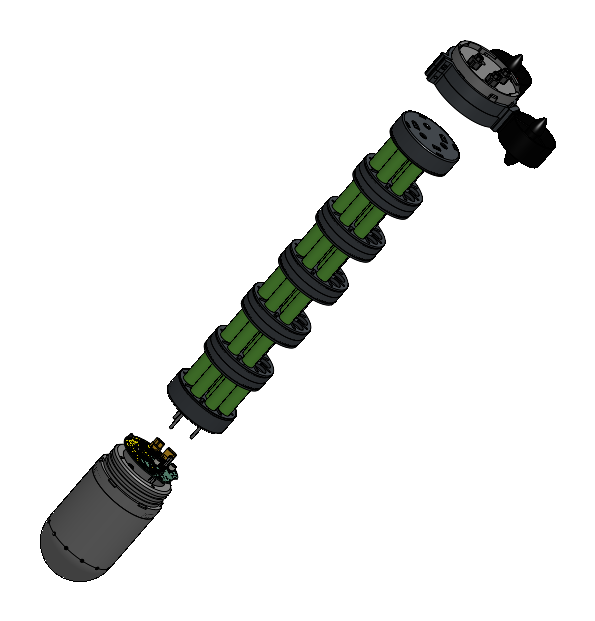
\includegraphics[width=\linewidth,height=52mm,keepaspectratio]{fabrication/cad_caiman_full_assembly.png}
    \caption{Vue d'ensemble 3D de l'assemblage complet du robot Caiman sous Onshape.}
  \end{subfigure}
  \hfill
  \begin{subfigure}[t]{0.48\textwidth}
    \centering
    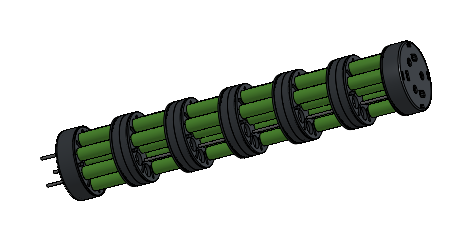
\includegraphics[width=\linewidth,height=52mm,keepaspectratio]{fabrication/cad_caiman_battery_pack.png}
    \caption{Structure du berceau interne et intégration du pack de batteries Li-ion 18650.}
  \end{subfigure}
  \caption{Modélisation CAO sous Onshape de la structure mécanique générale du Caiman.}
  \label{fig:caiman-cad-mechanics}
\end{figure}

La modélisation 3D illustre l'intégration compacte des sous-ensembles au sein du tube cylindrique étanche en polyméthacrylate de méthyle (PMMA). Ce matériau transparent a été retenu pour concilier une excellente résistance mécanique aux contraintes hydrostatiques et une visibilité directe sur la carte électronique Caiman et l'état des liaisons internes. Le berceau longitudinal maintient l'alignement des accumulateurs Li-ion 18650 ; la géométrie vise à centrer la masse afin de limiter les variations d'assiette en immersion, sans qu'un essai hydrostatique ait pu le vérifier.

\begin{figure}[htbp]
  \centering
  \begin{subfigure}[t]{0.48\textwidth}
    \centering
    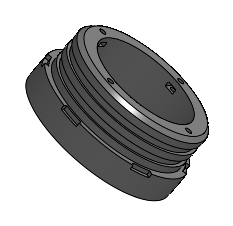
\includegraphics[width=\linewidth,height=48mm,keepaspectratio]{fabrication/cad_front_lid_clean.png}
    \caption{Flasque avant (\emph{Front Lid}) avec orifice du capteur Bar30 et hublot optique.}
  \end{subfigure}
  \hfill
  \begin{subfigure}[t]{0.48\textwidth}
    \centering
    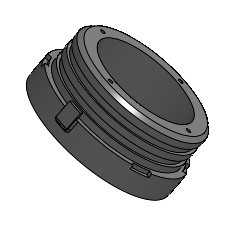
\includegraphics[width=\linewidth,height=48mm,keepaspectratio]{fabrication/cad_back_lid_clean.png}
    \caption{Flasque arrière (\emph{Back Lid}) équipée des pénétrateurs pour propulseurs T60.}
  \end{subfigure}
  \caption{Conception détaillée des flasques d'étanchéité avant et arrière du corps étanche.}
  \label{fig:caiman-lids-mechanics}
\end{figure}

Comme le montre la \cref{fig:caiman-lids-mechanics}, l'étanchéité radiale du tube repose sur deux flasques usinées en alu/polycarbonate intégrant une double gorge pour joint torique (O-ring). La flasque avant (\emph{Front Lid}) intègre le port du capteur de pression piézorésistif Bar30 ainsi que la réservation pour le dôme optique. La flasque arrière (\emph{Back Lid}) réunit les traversées étanches (\emph{bulkheads} hybrides M10) alimentant les deux propulseurs subaquatiques T60 ainsi que le câble de la balise radio de surface. La disposition axiale des pénétrateurs vise à limiter les pincements de câbles lors de la fermeture de l'enceinte.

\section{Contraintes de validation}

La réception tardive du PCB impose une stratégie par niveaux : vérification ERC/DRC des sources CAO, tests unitaires du logiciel de simulation, lecture et intégration statique du firmware, puis démonstration HIL du protocole sur des cartes de développement. Les essais d'alimentation, de programmation et de capteurs sur la carte Caiman restent hors du périmètre temporel du stage.

\section{Hypothèses de simulation et ordre de grandeur énergétique}

Le scénario par défaut du simulateur emploie cinq AUV, une batterie nominale de \SI{12}{\volt}/\SI{56}{\ampere\hour}, un courant moyen moteur de \SI{15}{\ampere} et une portée radio de surface de \SI{250}{\metre}. Ces valeurs sont des hypothèses de modélisation fournies au projet ; elles ne constituent ni des mesures sur le Caiman final ni des exigences qualifiées.

Elles permettent néanmoins un calcul d'ordre de grandeur facile à interpréter. L'énergie nominale et l'autonomie idéale limitée aux moteurs s'écrivent
\begin{align}
  E_{\mathrm{nom}} &= UQ
  = \SI{12}{\volt}\times\SI{56}{\ampere\hour}
  = \SI{672}{\watt\hour}, \\
  t_{\mathrm{idéal}} &= \frac{Q}{I_{\mathrm{moteurs}}}
  = \frac{\SI{56}{\ampere\hour}}{\SI{15}{\ampere}}
  \approx \SI{3.73}{\hour}.
\end{align}
Ce quotient sert uniquement de référence au modèle énergétique. Les pertes des convertisseurs, l'électronique, les pointes de man\oe{}uvre, l'environnement et la réserve de sécurité réduiraient l'autonomie réelle ; aucune durée de mission physique n'est donc revendiquée.

\chapter{Conception et revue de l'électronique}
\label{chap:hardware}

Les contraintes énoncées au \cref{chap:systeme} se traduisent, sur la carte, par un ensemble de choix de composants et de topologies. Ce chapitre en détaille la revue, en partant de la chaîne d'alimentation qui conditionne tout le reste.

\section{Architecture d'alimentation}

L'entrée d'alimentation est protégée par un contrôleur LM74700 avant deux conversions abaisseuses. Un AP63205 génère le rail \SI{5}{\volt}, puis un AP63203 génère le rail \SI{3.3}{\volt}. Les valeurs nominales prévues dans le schéma sont respectivement \SI{4.7}{\micro\henry} pour L1 et \SI{3.9}{\micro\henry} pour L2, conformément aux valeurs typiques proposées dans la documentation de la famille AP6320x \cite{diodes-ap6320x}.

La première nomenclature soumise à JLCPCB associait L1 au Vishay IHLP1616\-BZER4R7M5A et L2 au Sunlord SWPA4030\-S3R9MT. Le premier présente un courant de saturation typique de \SI{1.8}{\ampere} pour une diminution d'inductance d'environ 20\,\% \cite{vishay-ihlp1616}. Pour L2, le fabricant indique un courant de saturation minimal de \SI{3.0}{\ampere} et un courant thermique maximal de \SI{2.1}{\ampere} \cite{sunlord-swpa}. Faute de réception de la carte, ces valeurs restent des données de dimensionnement et non des mesures. Cette sélection a par la suite été revue lors de la préparation de l'assemblage, pour un motif géométrique développé au \cref{sec:inductances}.

La \cref{fig:pcb-3d} donne un aperçu de l'implantation obtenue après routage.

\subsection{Ondulation de courant dans les inductances}

Le modèle idéal d'un convertisseur abaisseur relie le rapport cyclique $D$, l'ondulation crête à crête $\Delta I_L$ et le courant de crête $I_{L,\mathrm{pic}}$ par
\begin{align}
  D &\simeq \frac{V_{\mathrm{out}}}{V_{\mathrm{in}}}, \\
  \Delta I_L &\simeq
    \frac{V_{\mathrm{out}}\left(1-D\right)}{L f_{\mathrm{sw}}}, \\
  I_{L,\mathrm{pic}} &\simeq I_{\mathrm{out}} + \frac{\Delta I_L}{2}.
  \label{eq:buck-ripple}
\end{align}
Les AP63203 et AP63205 commutent nominalement à \SI{1.1}{\mega\hertz} \cite{diodes-ap6320x}. En prenant \SI{12}{\volt} comme tension nominale en entrée de L1 et le rail \SI{5}{\volt} comme entrée de L2, le calcul donne les ordres de grandeur du \cref{tab:buck-ripple}.

\begin{table}[H]
  \centering
  \caption{Estimation idéale de l'ondulation des deux convertisseurs.}
  \label{tab:buck-ripple}
  \begin{tabular}{@{}lccccc@{}}
    \toprule
    & $V_{\mathrm{in}}$ & $V_{\mathrm{out}}$ & $L$ & $D$ & $\Delta I_L$ \\
    \midrule
    L1 / AP63205 & \SI{12}{\volt} & \SI{5}{\volt} & \SI{4.7}{\micro\henry} & 0,42 & \SI{0.56}{\ampere} \\
    L2 / AP63203 & \SI{5}{\volt} & \SI{3.3}{\volt} & \SI{3.9}{\micro\henry} & 0,66 & \SI{0.26}{\ampere} \\
    \bottomrule
  \end{tabular}
\end{table}

À la limite de \SI{2}{\ampere} annoncée pour le convertisseur, les pics idéaux seraient donc d'environ \SI{2.28}{\ampere} sur L1 et \SI{2.13}{\ampere} sur L2. Le premier dépasse le courant de saturation typique du composant alors retenu pour L1 (\SI{1.8}{\ampere}) : cela ne démontre pas une défaillance, car le courant réel du rail n'a pas été caractérisé, mais interdit de revendiquer une marge à \SI{2}{\ampere}. Le courant de charge visé, la température et la courbe d'inductance sous polarisation devront être vérifiés au bring-up.

\section{Microcontrôleur et bus}

Le STM32F765VITx centralise les interfaces. Le bus I\textsuperscript{2}C2 relie le LPS22HB, le LIS2MDL et le LSM6DSO, tandis qu'I\textsuperscript{2}C1 est exposé sur un connecteur séparé. Le nRF24 est raccordé à SPI1 avec les signaux CE, CSN et IRQ. La microSD utilise l'interface SDMMC et un contact de détection.

\begin{figure}[htbp]
  \centering
  \begin{subfigure}[t]{0.48\textwidth}
    \centering
    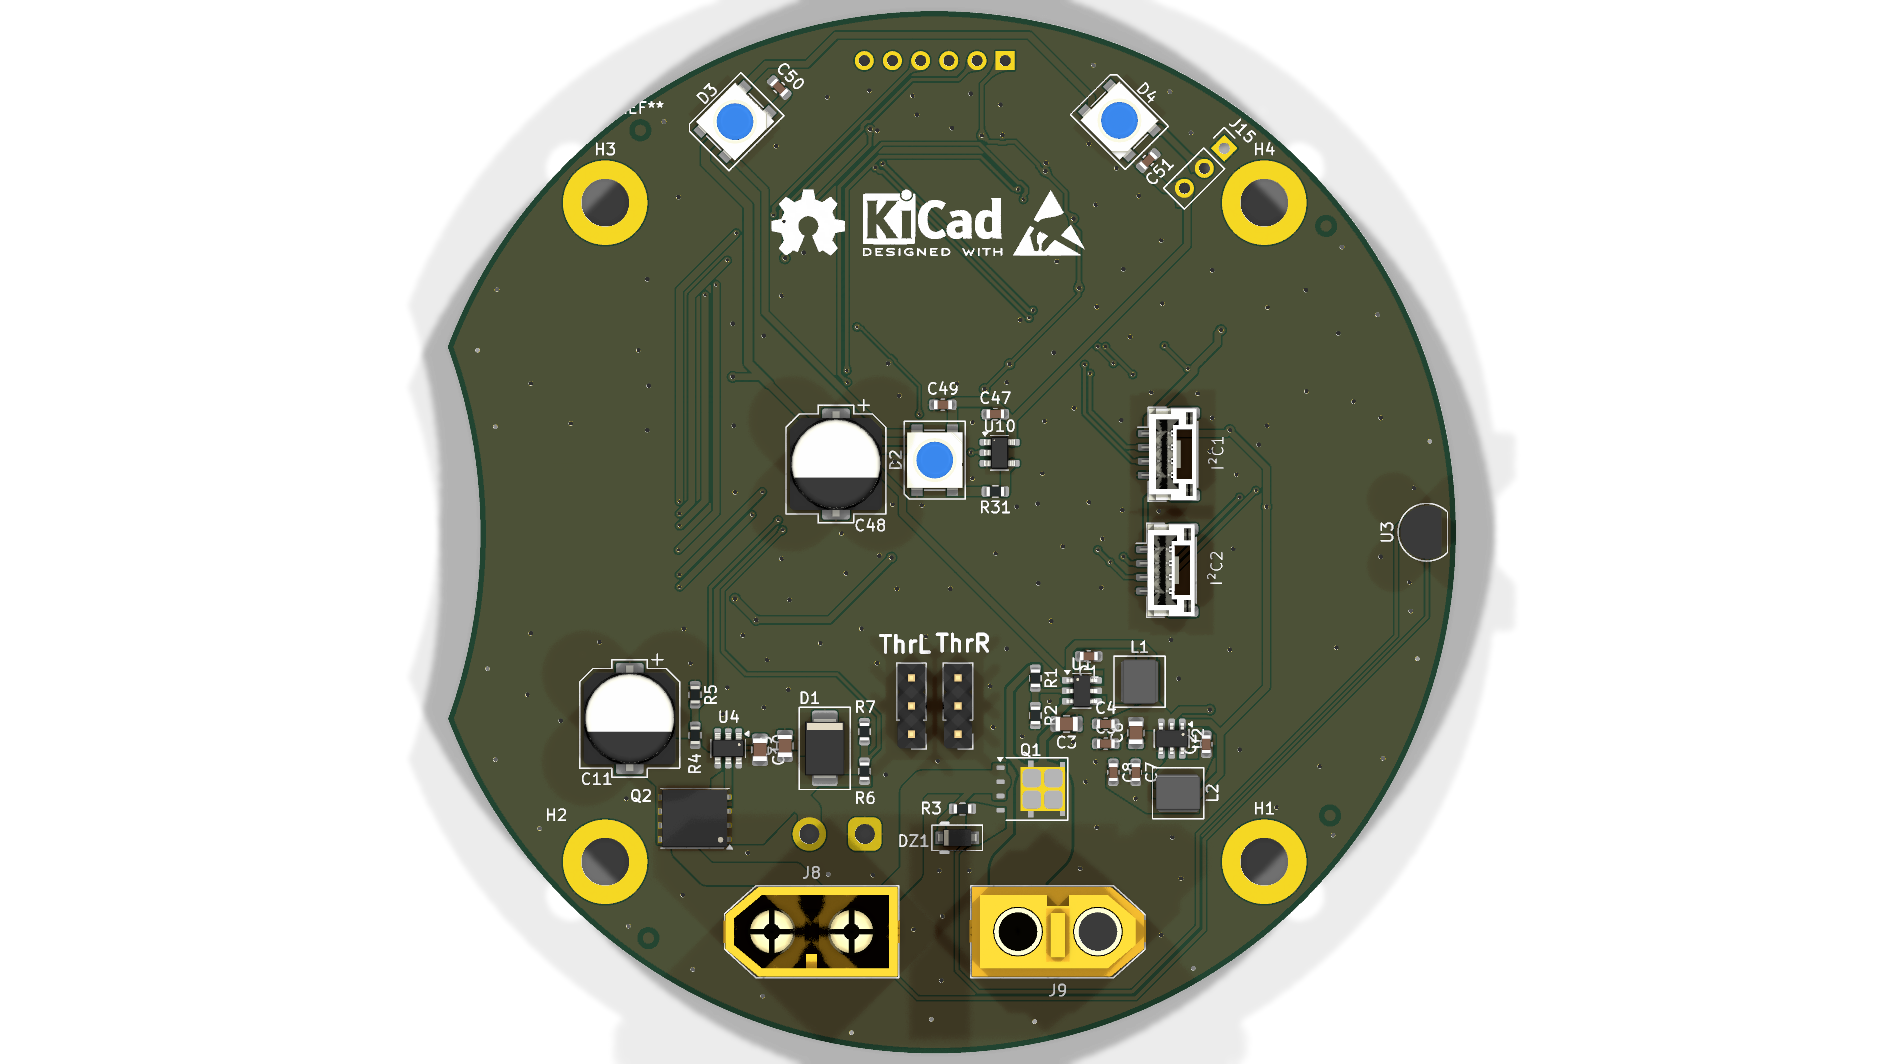
\includegraphics[width=\linewidth,height=52mm,keepaspectratio]{fabrication/pcb_3d_top.png}
    \caption{Vue de face de la carte (composants principaux).}
  \end{subfigure}
  \hfill
  \begin{subfigure}[t]{0.48\textwidth}
    \centering
    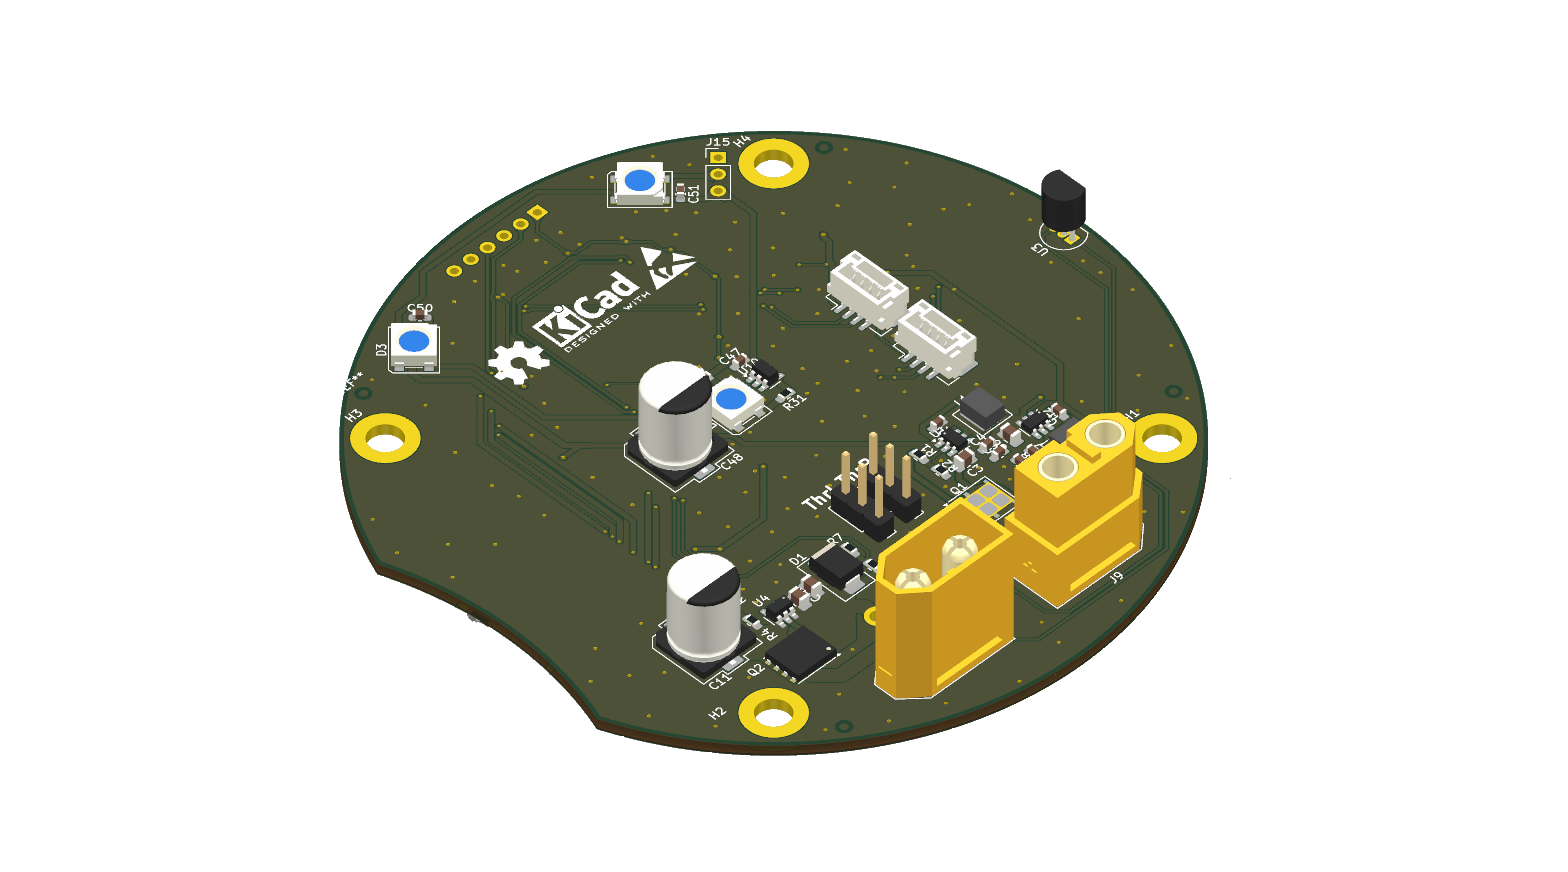
\includegraphics[width=\linewidth,height=52mm,keepaspectratio]{fabrication/pcb_3d_iso.png}
    \caption{Vue isométrique 3D calculée sous KiCad.}
  \end{subfigure}
  \caption{Rendu 3D de l'électronique Caiman généré depuis la révision KiCad du dépôt.}
  \label{fig:pcb-3d}
\end{figure}

\section{Corrections traçables et résolution d'anomalies de schéma}

L'audit approfondi du schéma hérité de la base amont et l'historique de versionnement Git mettent en évidence plusieurs corrections matérielles majeures indispensables au bon fonctionnement de la carte. La correction la plus critique de la révision électronique concerne le filtrage d'alimentation du STM32 (commit \GitCommit{dd041de}). Dans le schéma amont, les condensateurs de découplage de \SI{100}{\nano\farad} sur les lignes d'alimentation $V_{\mathrm{DD}}$, $V_{\mathrm{DDA}}$ et $V_{\mathrm{BAT}}$ du microcontrôleur STM32F765VITx étaient insérés par erreur en série sur les rails d'alimentation. Un condensateur en série se comportant comme un isolant en régime permanent (blocage du courant continu), cette topologie coupait l'arrivée de la tension \SI{3.3}{\volt} aux broches 11, 27, 50, 75, 100 et 71 du microcontrôleur, rendant son alimentation et son démarrage physiquement impossibles. La correction a consisté à replacer l'ensemble des condensateurs de découplage ($C_{12}$ à $C_{18}$) en parallèle entre le rail \SI{3.3}{\volt} et la masse (GND), rétablissant ainsi la continuité de l'alimentation DC tout en assurant le filtrage des parasites haute fréquence conformément au manuel de référence STMicroelectronics \cite{stmicro-stm32f765}. La \cref{fig:stm32-decoupling-comparison} compare les deux topologies.

Par ailleurs, la correction du type électrique de la masse du capteur inertiel LSM6DSO (commit \GitCommit{c66b3fb}) a résolu un conflit dans la matrice d'interconnexion KiCad causé par une broche de masse associée à une déclaration inadaptée. De même, la suppression des drapeaux d'alimentation superflus (commit \GitCommit{2be6335}) a permis d'assainir la déclaration des équipotentielles et la vérification des règles électriques. Grâce à ces interventions sur la saisie de schéma, les erreurs du vérificateur électrique (ERC) sous KiCad 10.0.5 passent de 10 erreurs bloquantes dans la révision initiale à zéro dans la version finale transmise à la fabrication, 42 avertissements mineurs subsistant. Le schéma complet après ces corrections est reproduit en \cref{app:evidence}, dans une taille permettant d'y localiser les points discutés ci-dessus.

\begin{figure}[htbp]
  \centering
  \begin{subfigure}[t]{0.92\textwidth}
    \centering
    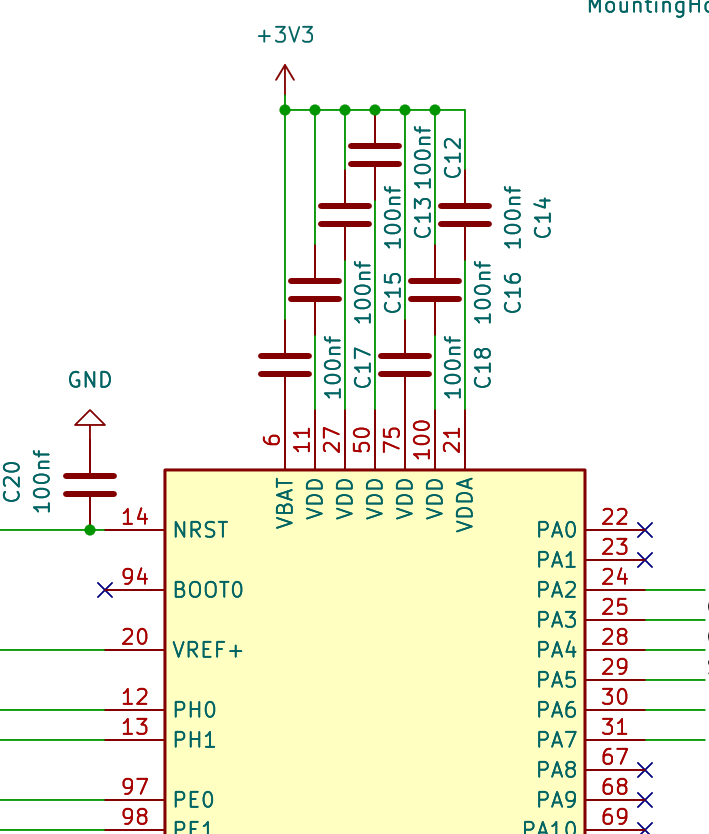
\includegraphics[width=\linewidth,height=98mm,keepaspectratio]{fabrication/stm32_decoupling_capacitors_before.png}
    \caption{Schéma amont hérité : condensateurs de \SI{100}{\nano\farad} en série sur les lignes $V_{\mathrm{DD}}$, ce qui bloque le courant continu.}
  \end{subfigure}

  \vspace{6mm}

  \begin{subfigure}[t]{0.92\textwidth}
    \centering
    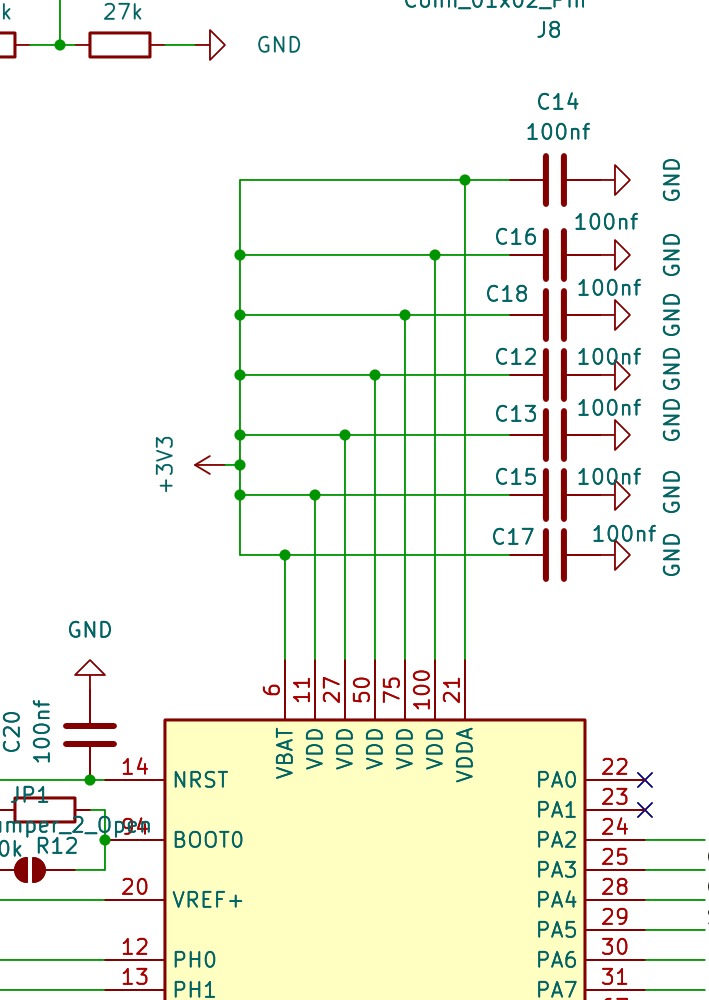
\includegraphics[width=\linewidth,height=98mm,keepaspectratio]{fabrication/stm32_decoupling_capacitors_fix.png}
    \caption{Schéma révisé (commit \GitCommit{dd041de}) : condensateurs replacés en parallèle entre le rail et la masse.}
  \end{subfigure}
  \caption{Comparaison avant/après de la correction du découplage d'alimentation du STM32 sous KiCad.}
  \label{fig:stm32-decoupling-comparison}
\end{figure}


\chapter{Routage et préparation à la fabrication}
\label{chap:fabrication}

\section{Vérification DRC et règles de fabrication}
\label{sec:drc}

Le contrôle des règles de conception (DRC) a fait l'objet de vérifications explicites tout au long du routage. Les règles du projet ont été alignées sur la grille de tolérances publiée par JLCPCB \cite{jlcpcb-capabilities}, avec une clearance cuivre interne de \SI{0.15}{\milli\metre}, une largeur de piste minimale de \SI{0.127}{\milli\metre} et un diamètre de via minimal de \SI{0.30}{\milli\metre}. Ces valeurs sont volontairement plus strictes que les capacités minimales du procédé, afin de conserver une marge industrielle.

Trois révisions successives ont été contrôlées : \GitCommit{654cd20} (8 juin 2026), \GitCommit{b900398} (9 juin 2026) et \GitCommit{b58eda6} (19 juin 2026). Sur cette dernière, le DRC ne signale plus qu'une seule violation résiduelle, reproductible avec la commande donnée en \cref{app:evidence}. Le \cref{tab:drc-final} récapitule cette violation et les écarts analysés puis documentés en exclusion.

\begin{table}[H]
  \centering
  \small
  \caption{Violations résiduelles analysées et documentées avant lancement en fabrication.}
  \label{tab:drc-final}
  \begin{tabularx}{\textwidth}{@{}l l X@{}}
    \toprule
    \textbf{Origine} & \textbf{Mesure} & \textbf{Analyse et décision} \\
    \midrule
    U5 --- \texttt{/I2C2\_SCL} / \texttt{GND} & \SI{0.1291}{\milli\metre} & Clearance interne au boîtier compact. Sous la règle de projet de \SI{0.15}{\milli\metre}, mais au-dessus du minimum piste/espacement publié de \SI{0.10}{\milli\metre} pour un cuivre \SI{1}{oz}. Exclusion documentée. \\
    U6 --- pad \texttt{NC} & --- & Pastille non connectée à proximité du plan \texttt{+3V3} ; sans fonction électrique, écart accepté. \\
    U8 --- pad \texttt{INT2} & \SI{0.1472}{\milli\metre} & Pastille non connectée ; écart de \SI{2.8}{\micro\metre} sous la règle interne, très au-dessus de la capacité du procédé. \\
    U2 --- \texttt{BST} / \texttt{SW} & \SI{0.132}{\milli\metre} & Broches adjacentes du convertisseur, empreinte constructeur imposée. \\
    \bottomrule
  \end{tabularx}
\end{table}

Toutes ces occurrences relèvent de la même catégorie : des écarts entre une règle interne conservatrice et la géométrie imposée par des empreintes de composants compacts, chacun restant au-dessus des capacités publiées du fabricant. Aucune ne correspond à une impossibilité de fabrication. Elles ont été inscrites dans la liste d'exclusions du projet plutôt que masquées par un abaissement global des règles, afin que le motif de chaque acceptation reste consultable dans le fichier de projet.

Le dossier de production a ensuite été soumis à la revue DFM du fabricant avant le lancement, étape qui a également conduit à la reprise des inductances de puissance décrite en \cref{sec:inductances}.

Le PCB ayant été commandé mais non reçu à la date de rédaction, une inspection visuelle et un contrôle de continuité des rails d'alimentation seront réalisés à la réception, préalablement à toute mise sous tension.

Un enseignement méthodologique se dégage de cette phase : le DRC gagne à être traité comme une condition de sortie de l'export de production, réexécuté sur l'état exact qui alimente les fichiers transmis, et non comme une étape franchie une fois pour toutes en cours de routage. La trace de cette exécution mérite d'être archivée avec la commande.

\section{Dossier de production}

Le dossier comprend les Gerbers des deux couches cuivre, les masques de soudure, les sérigraphies, le contour de carte et les perçages PTH/NPTH. La nomenclature sélectionnée (BOM) référence 116 composants placés.

La commande JLCPCB du 23 juin 2026 porte sur cinq cartes FR-4 TG135 de \SI{100.87}{\milli\metre} par \SI{93.94}{\milli\metre}, deux couches, cuivre externe \SI{1}{oz}, finition ENIG, masque noir, sérigraphie blanche et vias tented. Le fabricant annonce un test électrique flying-probe et une conformité IPC classe 2 ; la \cref{fig:jlc-order-details} en reproduit le récapitulatif. L'épaisseur commandée est \SI{0.8}{\milli\metre}, alors que le stackup du fichier KiCad reste configuré à \SI{1.6}{\milli\metre}. Cette différence n'affecte pas la comparaison des clearances cuivre à \SI{1}{oz}, mais elle doit être prise en compte pour la rigidité mécanique, la fixation et les connecteurs.

\begin{figure}[htbp]
  \centering
  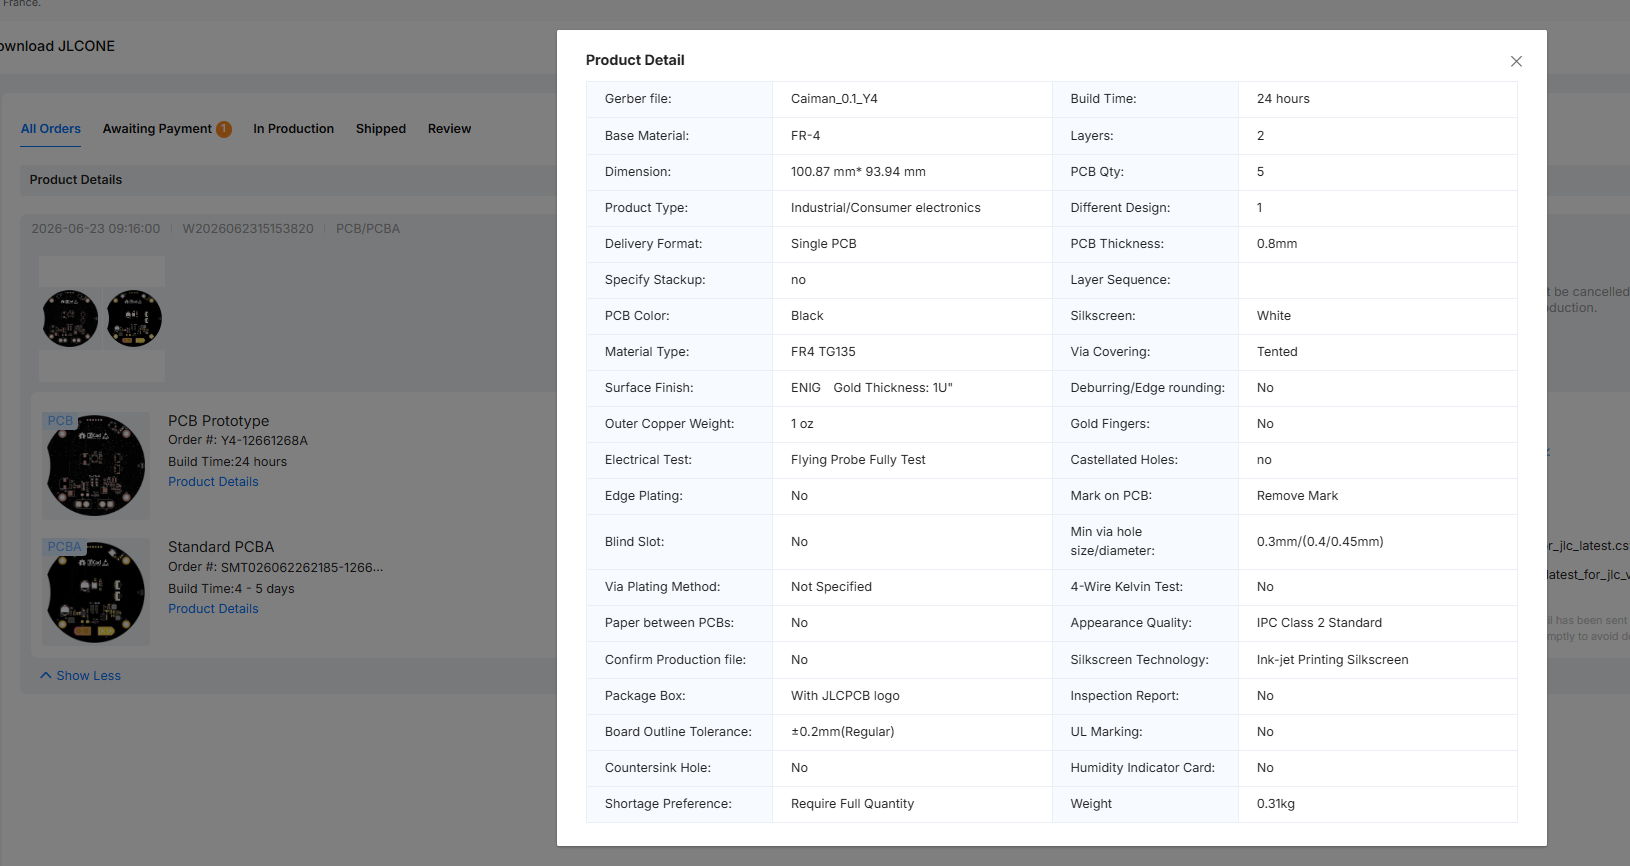
\includegraphics[width=0.9\textwidth,height=0.35\textheight,keepaspectratio]{fabrication/jlcpcb_order_details_2026-06-23.png}
  \caption{Détails de la commande PCB JLCPCB du 23 juin 2026.}
  \label{fig:jlc-order-details}
\end{figure}

\begin{figure}[htbp]
  \centering
  \begin{subfigure}[t]{0.48\textwidth}
    \centering
    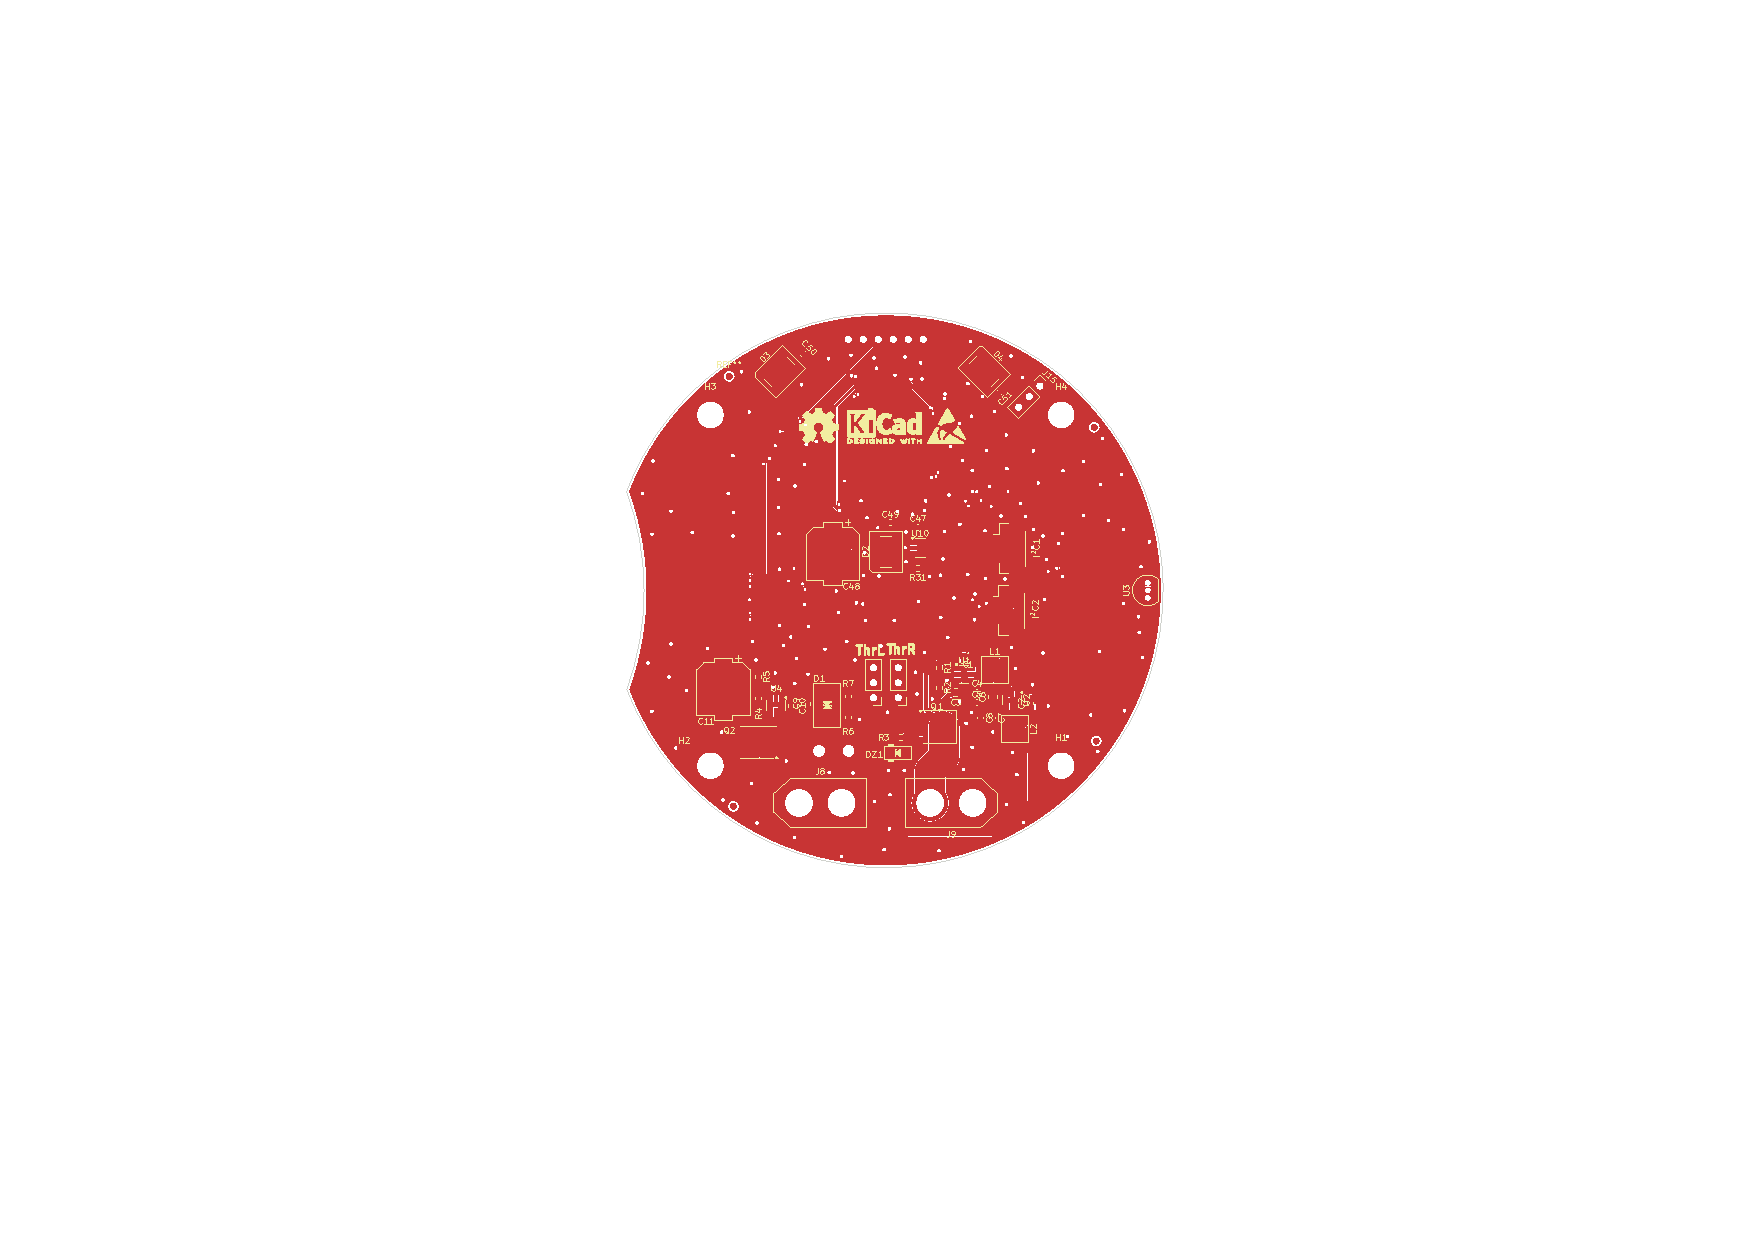
\includegraphics[width=\linewidth]{fabrication/pcb_routing_top_cropped.pdf}
    \caption{Couche supérieure (F.Cu) : bus, alimentation et empreintes CMS.}
  \end{subfigure}
  \hfill
  \begin{subfigure}[t]{0.48\textwidth}
    \centering
    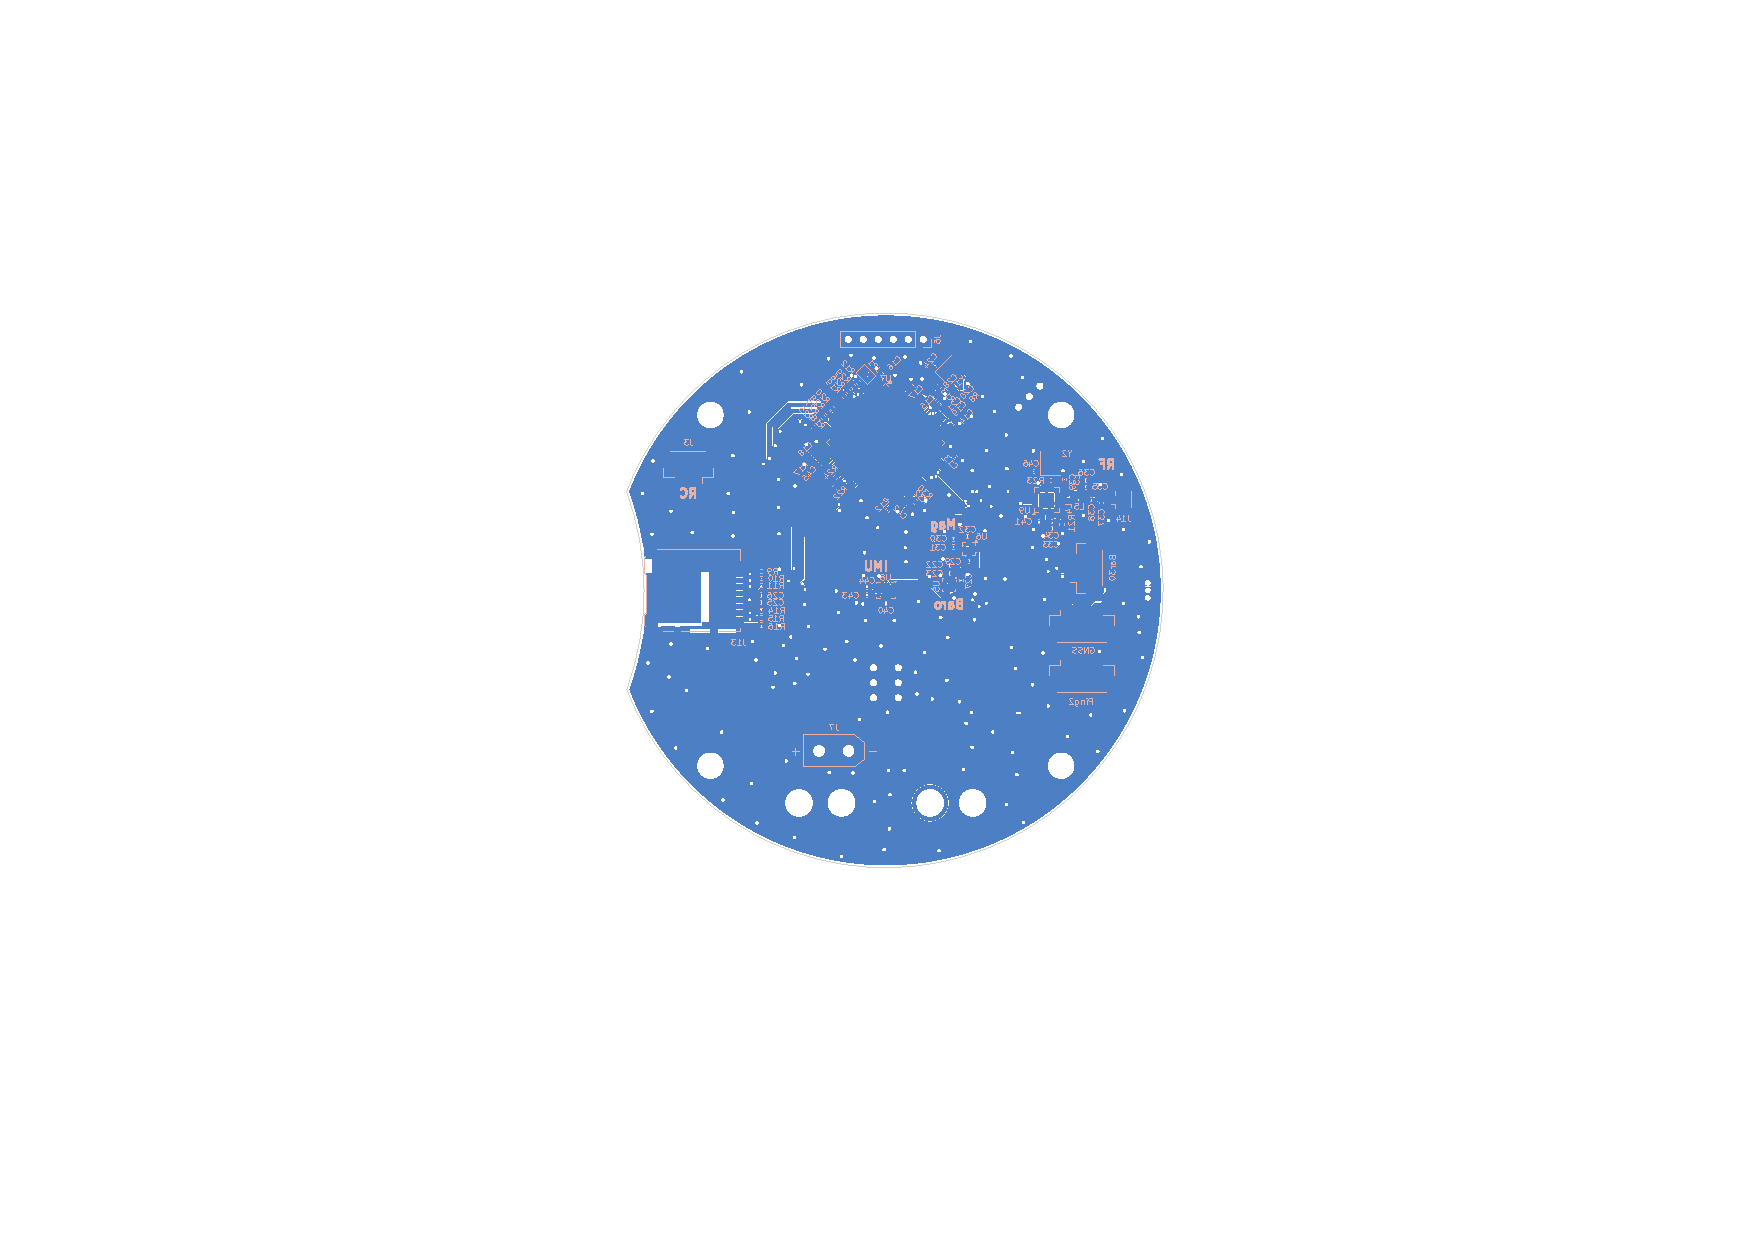
\includegraphics[width=\linewidth]{fabrication/pcb_routing_bottom_cropped.pdf}
    \caption{Couche inférieure (B.Cu) : plan de masse et découplage.}
  \end{subfigure}
  \caption{Plans de routage haute résolution de la carte Caiman (revue de fabrication).}
  \label{fig:pcb-routing-composite}
\end{figure}

Les deux couches cuivre telles que transmises sont reproduites en \cref{fig:pcb-routing-composite}. La carte n'étant pas encore reçue à la date de rédaction du rapport, ni la qualité d'assemblage ni le fonctionnement électrique sur le PCB physique ne sont validés.

\section{Sélection finale et remplacement des inductances de puissance (L1 et L2)}
\label{sec:inductances}

Lors de la préparation du fichier PCBA pour l'assemblage automatisé SMT chez JLCPCB, la revue d'ingénierie du fabricant a révélé une incompatibilité géométrique entre l'empreinte (\emph{land pattern}) dessinée sur la carte et la géométrie des plages de brasage des composants initialement présélectionnés dans la nomenclature. Le fabricant a suspendu l'assemblage et proposé quatre options : re-sélectionner un composant compatible, laisser les emplacements non peuplés, annuler la commande, ou braser en l'état sans garantie. La \cref{fig:jlc-inductances} reproduit cet échange et la superposition des empreintes qui l'accompagne.

\begin{figure}[htbp]
  \centering
  \begin{subfigure}[t]{\textwidth}
    \centering
    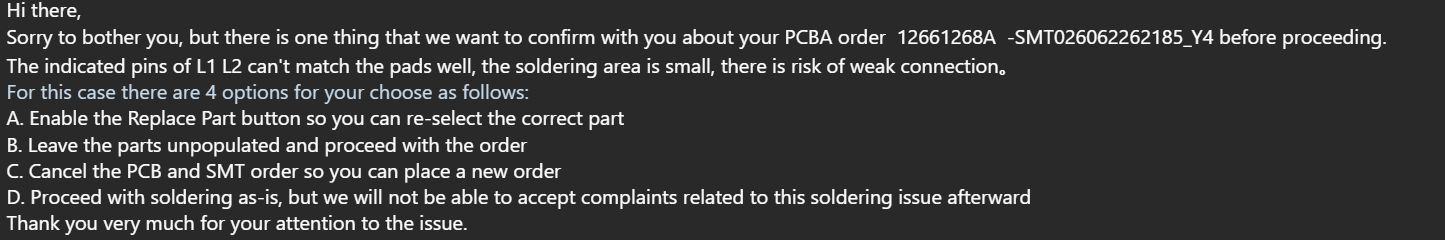
\includegraphics[width=\linewidth]{fabrication/jlcpcb_pcba_L1L2_message.png}
    \caption{Signalement de la revue PCBA : surface de brasage insuffisante sur L1 et L2.}
  \end{subfigure}

  \vspace{4mm}

  \begin{subfigure}[t]{0.52\textwidth}
    \centering
    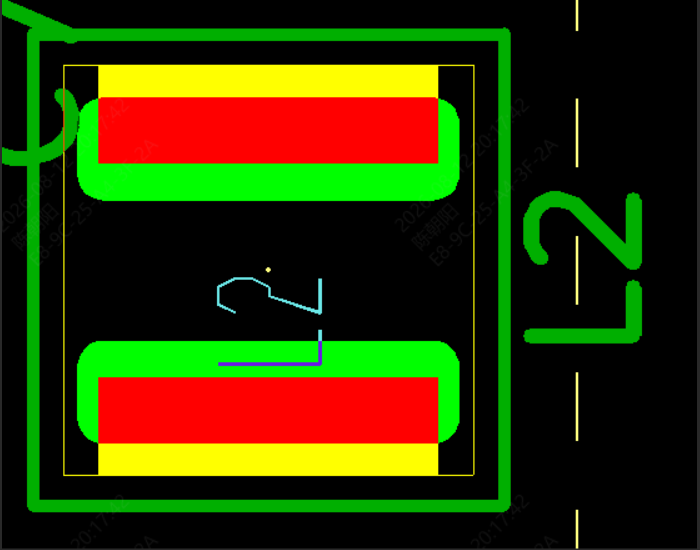
\includegraphics[width=\linewidth]{fabrication/jlcpcb_pcba_L1L2_pads.png}
    \caption{Superposition des plages de la carte (contour vert) et des terminaisons du composant proposé (zones rouges), montrant le débord latéral.}
  \end{subfigure}
  \caption{Détection d'une incompatibilité géométrique lors de la revue PCBA du 12 août 2026 et bascule vers des références correspondant au land pattern WE-MAPI 4020.}
  \label{fig:jlc-inductances}
\end{figure}

L'option retenue a été la re-sélection des composants : elle seule préserve à la fois la fonction des deux convertisseurs et la fiabilité mécanique du joint brasé. Les références finalement commandées sont données au \cref{tab:inductors-selection}.

Ce décalage met en évidence un enseignement fondamental en ingénierie électronique : des dimensions extérieures de boîtier identiques (ex. $4\times4\,\text{mm}$) ne garantissent en aucun cas une compatibilité de routage ou d'empreinte sous le composant. La sélection finale a été entièrement reprise en comparant les datasheets constructeurs, les valeurs d'inductance, le courant thermique nominal, le courant de saturation, la résistance DC (DCR) et la géométrie exacte des pads.

\begin{table}[htbp]
  \centering
  \small
  \caption{Spécifications finales des inductances de puissance sélectionnées pour l'assemblage PCBA.}
  \label{tab:inductors-selection}
  \begin{tabularx}{\textwidth}{@{}l c l l c r@{}}
    \toprule
    \textbf{Désignateur} & \textbf{Valeur} & \textbf{Empreinte} & \textbf{Référence fabricant} & \textbf{Code LCSC} & \textbf{Courant sat.} \\
    \midrule
    L1 (Buck 5V) & \SI{4.7}{\micro\henry} & WE-MAPI 4020 & Würth 74438356047 & C2045367 & \SI{2.5}{\ampere} \\
    L2 (Buck 3.3V) & \SI{3.3}{\micro\henry} & WE-MAPI 4020 & Würth 74438356033 & C2045382 & \SI{3.0}{\ampere} \\
    \bottomrule
  \end{tabularx}
\end{table}

Pour le régulateur Buck 3,3\,V (AP63203), le schéma initial spécifiait une valeur nominale de \SI{3.9}{\micro\henry}. Pour l'assemblage réel, l'inductance retenue en boîtier WE-MAPI 4020 est de \SI{3.3}{\micro\henry} (Würth \texttt{74438356033}). Selon la spécification constructeur Diodes Inc. AP63203 \cite{diodes-ap6320x}, la plage d'inductance recommandée s'étend de \SI{2.2}{\micro\henry} à \SI{10}{\micro\henry} pour un courant de sortie jusqu'à \SI{2}{\ampere}. La valeur de \SI{3.3}{\micro\henry} maintient une ondulation de courant acceptable tout en accélérant la réponse dynamique lors des appels de courant des sous-systèmes radio et capteurs.

Ce changement de valeur impose de reprendre l'estimation d'ondulation conduite au \cref{chap:hardware}, qui utilisait la valeur nominale du schéma. En appliquant l'\cref{eq:buck-ripple} aux composants finalement retenus, on obtient les marges du \cref{tab:inductors-margins}.

\begin{table}[H]
  \centering
  \small
  \caption{Ondulation et courant de crête recalculés pour les inductances effectivement sélectionnées, à la charge maximale annoncée de \SI{2}{\ampere}.}
  \label{tab:inductors-margins}
  \begin{tabular}{@{}lccccc@{}}
    \toprule
    & $L$ retenue & $D$ & $\Delta I_L$ & $I_{L,\mathrm{pic}}$ & $I_{\mathrm{sat}}$ \\
    \midrule
    L1 / AP63205 & \SI{4.7}{\micro\henry} & 0,42 & \SI{0.56}{\ampere} & \SI{2.28}{\ampere} & \SI{2.5}{\ampere} \\
    L2 / AP63203 & \SI{3.3}{\micro\henry} & 0,66 & \SI{0.31}{\ampere} & \SI{2.16}{\ampere} & \SI{3.0}{\ampere} \\
    \bottomrule
  \end{tabular}
\end{table}

Deux lectures en découlent. Sur L2, le passage de \SI{3.9}{} à \SI{3.3}{\micro\henry} augmente l'ondulation d'environ \SI{18}{\percent}, mais le courant de crête reste largement en dessous de la saturation de la référence Würth retenue : la substitution ne dégrade pas la marge. Sur L1, en revanche, le courant de crête idéal approche la saturation publiée à moins de \SI{10}{\percent} près. La réserve formulée au \cref{chap:hardware} sur ce rail subsiste donc après la nouvelle sélection : elle n'établit pas une défaillance, puisque le courant réellement consommé par le rail \SI{5}{\volt} n'a pas été caractérisé, mais elle interdit de revendiquer une marge confortable à pleine charge. La mesure du courant de rail et le relevé de la courbe d'inductance sous polarisation figurent parmi les premiers contrôles à conduire au bring-up.


\chapter{Logiciel embarqué}
\label{chap:software}

La carte étant partie en fabrication, le travail logiciel a pu progresser en parallèle, sans toutefois pouvoir être éprouvé sur la cible. Le firmware repose sur STM32Cube et FreeRTOS. La tâche principale appelle l'initialisation de la couche applicative capteurs, puis exécute périodiquement sa fonction de service. La période visée est d'environ \SI{100}{\milli\second}, soit \SI{10}{\hertz}. Le \cref{tab:drivers} situe le niveau de maturité atteint par chaque fonction.

\section{Niveaux de maturité}

\begin{table}[H]
  \centering
  \caption{État des principales fonctions logicielles à la fin du stage.}
  \label{tab:drivers}
  \begin{tabularx}{\textwidth}{@{}>{\raggedright\arraybackslash}p{0.24\textwidth} c c c >{\raggedright\arraybackslash}X@{}}
    \toprule
    \textbf{Fonction} & \textbf{Code} & \textbf{Intégrée} & \textbf{Test PCB} & \textbf{Observation} \\
    \midrule
    LSM6DSO, LIS2MDL, LPS22HB & oui & oui & non & Lecture prévue dans la tâche capteurs. \\
    Batterie ADC, RGB, microSD & oui & oui & non & Logger intégré ; format CSV à harmoniser. \\
    nRF24, ESC, Bar30 & oui & non & non & Pilotes présents, hors chemin applicatif principal audité. \\
    GNSS, Ping2, RC, fuite, contact magnétique & partiel & non & non & Squelettes ou stubs. \\
    \bottomrule
  \end{tabularx}
\end{table}

Aucun de ces pilotes n'a été validé sur le PCB Caiman, la carte n'ayant pas été reçue. Le résultat du stage est donc une base logicielle destinée au premier bring-up, et non un firmware de production qualifié.

Une incohérence a été identifiée dans la journalisation : l'en-tête CSV annonce dix colonnes tandis que l'application écrit dix-huit champs. Ce point devra être corrigé avant l'exploitation des mesures.

\section{Essai exploratoire STM32 et centrale inertielle}

En parallèle du firmware cible, un premier banc a été réalisé avec une carte NUCLEO-H743ZI2 et un module SparkFun Qwiic 9DoF fondé sur l'ICM-20948. Ce banc, reproduit en \cref{fig:stm32-imu-exploratory}, avait pour objectif de se familiariser avec une chaîne d'acquisition inertielle sur STM32 et d'identifier les besoins futurs de navigation du sous-marin : mesure des accélérations et vitesses angulaires, information de cap, calibration et fusion ultérieure avec la profondeur et les positions disponibles en surface.

Les essais ont fourni une première observation qualitative du comportement d'une centrale inertielle au repos et lors de mouvements du module. Ils ont surtout servi à préparer la démarche d'intégration : alimentation et raccordement d'un capteur externe, initialisation, lecture périodique et interprétation des axes. Aucun journal brut, graphique temporel ni protocole métrologique n'étant conservé avec les photographies, aucune précision, fréquence ou dérive chiffrée n'est revendiquée.

\begin{figure}[htbp]
  \centering
  \begin{subfigure}[t]{0.47\textwidth}
    \centering
    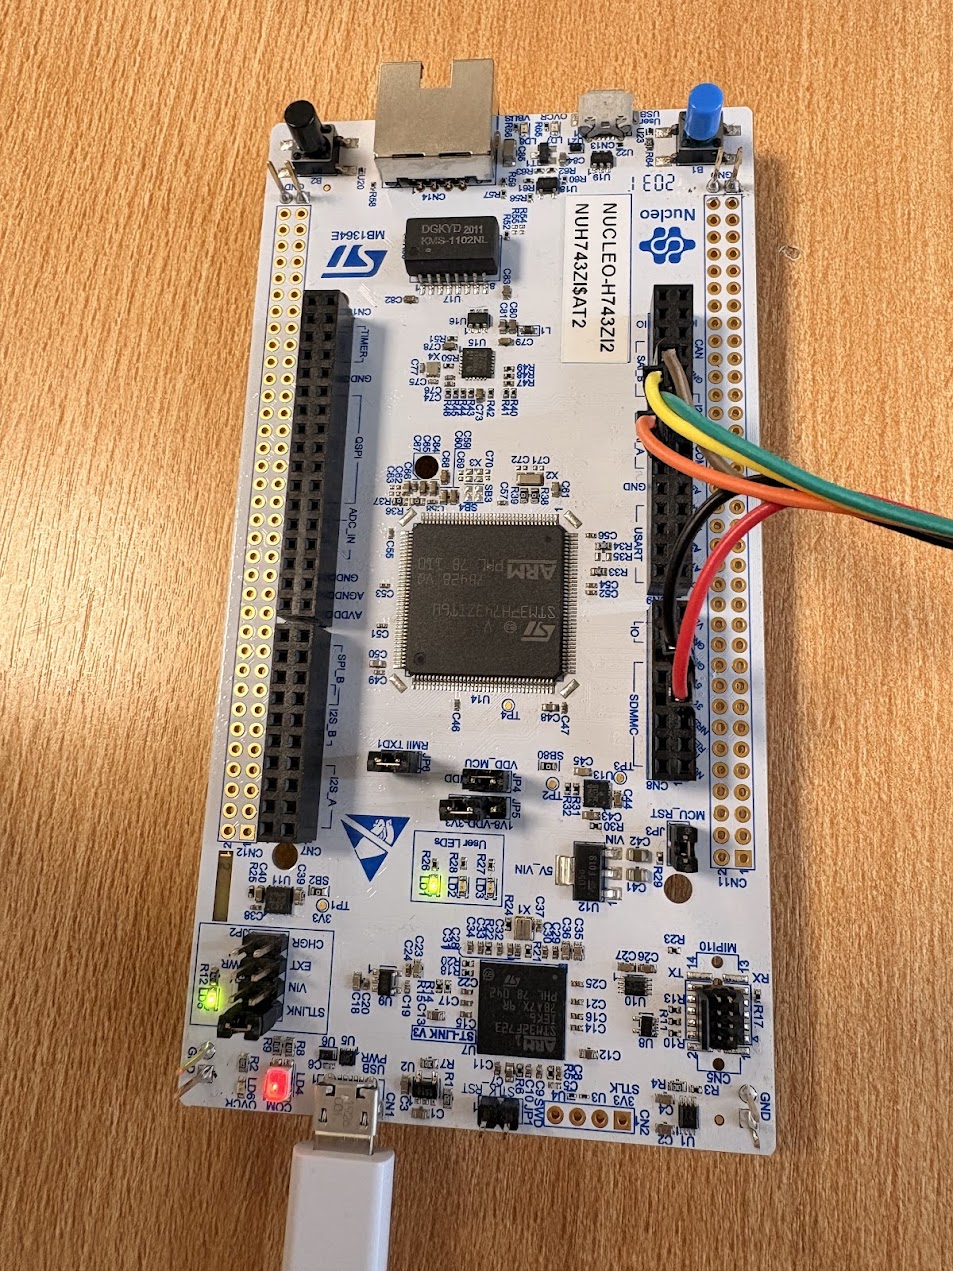
\includegraphics[height=64mm]{stm32/nucleo_h743zi2_banc_2026-06-10.jpg}
    \caption{Carte NUCLEO-H743ZI2 alimentée et raccordée par fils de prototypage.}
  \end{subfigure}\hfill
  \begin{subfigure}[t]{0.47\textwidth}
    \centering
    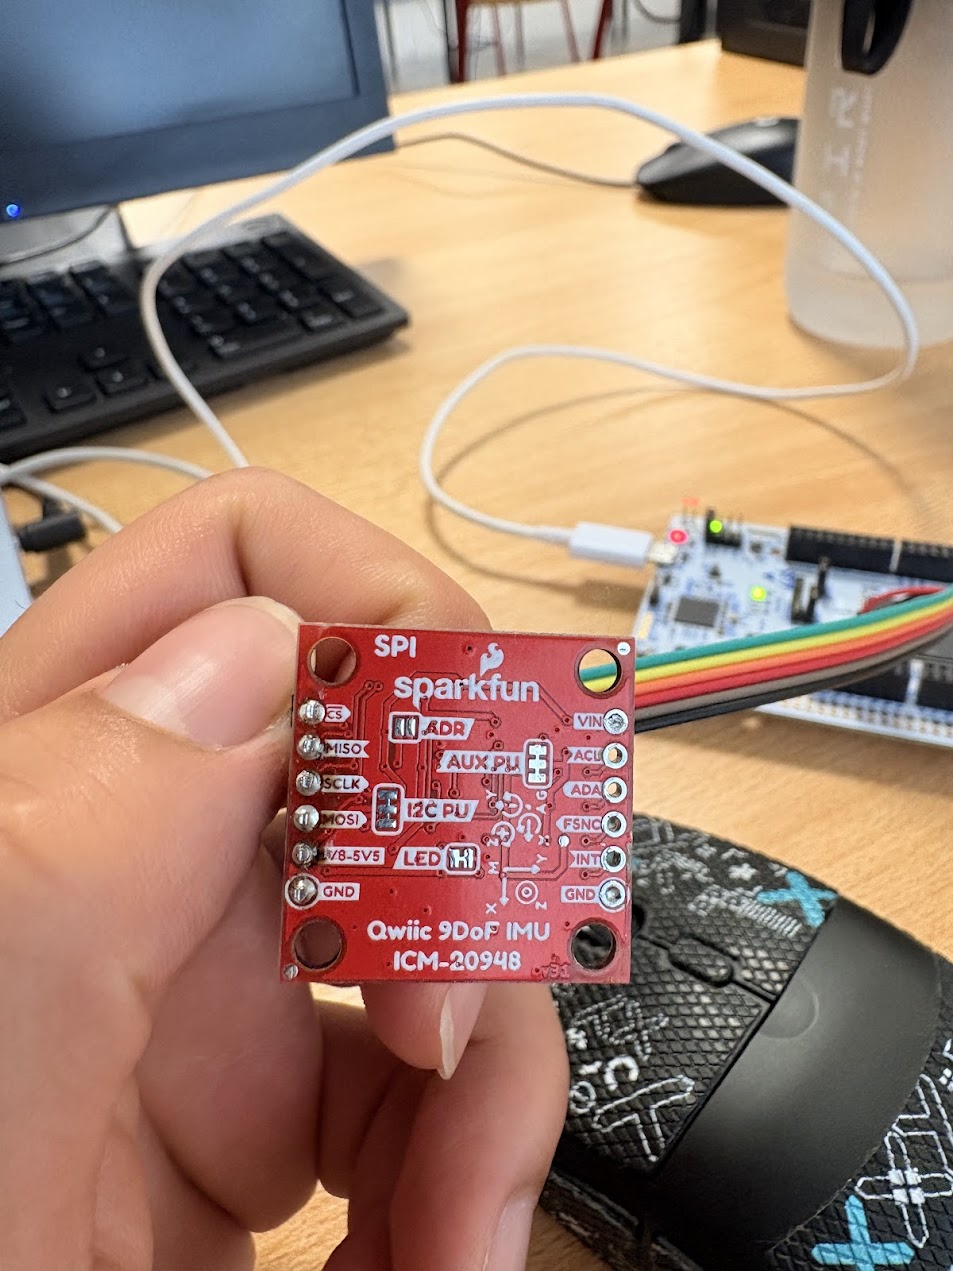
\includegraphics[height=64mm]{stm32/imu_icm20948_detail_2026-06-10.jpg}
    \caption{Module neuf axes ICM-20948 utilisé pour les essais.}
  \end{subfigure}
  \caption{Banc exploratoire STM32/IMU réalisé avant la disponibilité de la carte Caiman.}
  \label{fig:stm32-imu-exploratory}
\end{figure}

Ce prototype diffère du matériel final : la NUCLEO utilise un STM32H743, alors que Caiman est fondée sur un STM32F765VITx \cite{stmicro-stm32f765} et sépare la fonction inertielle entre LSM6DSO et LIS2MDL. Il démontre donc une prise en main et une intention d'architecture, pas la validation des pilotes ni des performances du PCB Caiman.

\subsection{Repère théorique pour l'estimation d'attitude}

L'exploitation future des mesures peut s'appuyer sur un filtre complémentaire ou un observateur d'attitude sur SO(3), modèles fondamentaux en automatique, estimation et navigation robotique \cite{mahony2008nonlinear, madgwick2011estimation}. Pour un angle de roulis ou de tangage, une écriture discrète est
\begin{equation}
  \widehat{\theta}_k =
  \alpha\left(\widehat{\theta}_{k-1}+\omega_{g,k}\Delta t\right)
  +(1-\alpha)\theta_{a,k},
  \qquad 0<\alpha<1,
  \label{eq:complementary-filter}
\end{equation}
où $\omega_{g,k}$ est la vitesse angulaire mesurée par le gyroscope, $\Delta t$ la période d'échantillonnage et $\theta_{a,k}$ l'inclinaison déduite de la direction de la gravité mesurée par l'accéléromètre. Le premier terme suit rapidement le mouvement mais accumule une dérive ; le second fournit une référence lente, plus sensible aux accélérations parasites. Leur pondération combine donc deux informations complémentaires \cite{narkhede-complementary-filter}.

Cette équation formalise une perspective, pas un résultat du banc photographié : aucun coefficient $\alpha$, aucune calibration et aucune précision d'attitude n'ont été validés. L'estimation du cap demanderait en outre le magnétomètre et sa calibration dans l'environnement magnétique du véhicule.

\chapter{Simulation de mission, supervision et communication sécurisée}
\label{chap:communication}

\section{Objectifs et périmètre}

Le délai de fabrication du PCB ne permettait pas d'attendre la carte finale pour étudier le comportement d'une flotte. Un simulateur déterministe a donc été développé afin d'éprouver la logique de mission collective, les contraintes de communication, la supervision, les défauts et la sécurité indépendamment du matériel. Il ne cherche pas à reproduire l'hydrodynamique complète d'un AUV : il constitue un banc d'étude de niveau système, observable et reproductible.

Les objectifs principaux sont les suivants :

\begin{itemize}
  \item distribuer une mission bathymétrique entre plusieurs véhicules ;
  \item représenter la perte totale du lien radio lorsqu'un robot est immergé ;
  \item distinguer l'état interne du modèle des informations réellement reçues par le navire ;
  \item étudier le stockage différé, les rendez-vous de surface et les relais multi-sauts ;
  \item spécifier une trame compatible avec la limite physique de 32 octets du nRF24 ;
  \item tester chiffrement, authentification, anti-rejeu, rotation de clé, commandes et injections de défauts ;
  \item fournir une interface de démonstration et des exports exploitables hors du programme.
\end{itemize}

La graine pseudo-aléatoire, les paramètres de flotte et le profil de communication sont explicitement configurables. Deux exécutions utilisant les mêmes paramètres produisent ainsi les mêmes décisions de mission et permettent de comparer les effets d'une perte, d'une portée ou d'un défaut différent.

\section{Architecture logicielle}

L'application est écrite en Python et séparée en composants spécialisés, dont la \cref{fig:sim-architecture} donne l'organisation. L'interface Streamlit ne réalise ni chiffrement ni décision de routage : elle configure le modèle, avance son horloge discrète et affiche des instantanés publics. Cette séparation évite de confondre logique métier et représentation graphique.

\begin{figure}[htbp]
  \centering
  \resizebox{\textwidth}{!}{%
  \begin{tikzpicture}[
      node distance=7mm and 8mm,
      block/.style={draw=enstablue, rounded corners, align=center, fill=blue!4,
                    minimum height=8mm, text width=30mm, font=\small},
      wide/.style={block, text width=48mm},
      arrow/.style={-{Latex[length=2mm]}, thick, draw=caimanblue}
    ]
    \node[wide] (ui) {Interface Streamlit\\paramètres et vues opérateur};
    \node[wide, below=of ui] (sim) {Coordinateur de simulation\\horloge et états de mission};
    \node[block, below left=10mm and 39mm of sim] (robot) {Robots\\mouvement, énergie, commandes};
    \node[block, below left=10mm and 3mm of sim] (bathy) {Bathymétrie\\terrain, sonar, trajectoires};
    \node[block, below right=10mm and 3mm of sim] (network) {Réseau\\portée, pertes, flooding};
    \node[block, below right=10mm and 39mm of sim] (security) {Protocole\\codec, clés, anti-rejeu};
    \node[wide, below=21mm of sim] (logs) {Événements, télémétrie et paquets\\exports CSV et JSON};
    \draw[arrow] (ui) -- (sim);
    \draw[arrow] (sim) -- (robot);
    \draw[arrow] (sim) -- (bathy);
    \draw[arrow] (sim) -- (network);
    \draw[arrow] (sim) -- (security);
    \draw[arrow] (robot) -- (logs);
    \draw[arrow] (bathy) -- (logs);
    \draw[arrow] (network) -- (logs);
    \draw[arrow] (security) -- (logs);
  \end{tikzpicture}%
  }
  \caption{Architecture fonctionnelle du simulateur Caiman.}
  \label{fig:sim-architecture}
\end{figure}

Le coordinateur orchestre les modèles de robots, la bathymétrie, le réseau, la station de base et les événements. Le transport est abstrait derrière une même interface : les profils nRF24 de surface, maillage idéal et modems acoustiques exploratoires réutilisent donc la même mission. Cette organisation prépare également le remplacement ultérieur d'un lien simulé par un adaptateur série, UDP ou radio réel.

\section{Mission bathymétrique coordonnée}

La configuration par défaut contient cinq AUV dans une zone de calcul de \SI{1000}{\metre} par \SI{700}{\metre}. Le polygone effectivement levé couvre environ \SI{0.32}{\square\kilo\metre} et le fond synthétique évolue approximativement entre \SI{13}{\metre} et \SI{20}{\metre}. Pour une graine donnée, le terrain reste identique ; il combine pente, bassin, haut-fond, chenal et relief lissé. Il ne s'agit pas d'un relevé hydrographique réel.

Au déploiement, les transects boustrophédon sont répartis entre tous les robots. Chaque véhicule suit une consigne située environ trois mètres au-dessus du fond virtuel, mesure un sonar mono-faisceau de \ang{25} et conserve ses échantillons à bord pendant l'immersion. À cette altitude, l'empreinte physique représentée est de l'ordre de \SI{1.3}{\metre} ; le pourcentage cartographié par le PC correspond toutefois à une grille de reconnaissance soutenue par une trajectoire mesurée à moins de \SI{26}{\metre}, et non à une insonification directe de chaque mètre carré.

La largeur géométrique $d_f$ de l'empreinte d'un faisceau conique d'ouverture $\beta$ à une hauteur $h$ s'obtient par une simple trigonométrie :
\begin{equation}
  d_f = 2h\tan\left(\frac{\beta}{2}\right)
  = 2\times\SI{3}{\metre}\times\tan(\ang{12.5})
  \approx \SI{1.33}{\metre}.
  \label{eq:sonar-footprint}
\end{equation}
L'ouverture de \ang{25} correspond à la documentation du sonar Ping \cite{bluerobotics-ping}. Ce calcul, directement relié à la navigation robotique, explique pourquoi une carte continue exige interpolation et recouvrement des trajectoires.

Le cycle de mission suit cinq étapes :

\begin{enumerate}
  \item départ du navire et descente vers les transects assignés ;
  \item levé autonome avec journalisation locale ;
  \item rendez-vous de surface, les arrivées anticipées réalisant de petites patrouilles sonar ;
  \item fusion des mesures datées et départ immédiat vers le bloc suivant ;
  \item passe coopérative de fermeture des lacunes, retour au navire et déchargement final.
\end{enumerate}

Tous les AUV participent au levé et deviennent des porteurs de données redondants lors des contacts. La version actuelle n'immobilise donc aucun véhicule dans un rôle permanent de \enquote{mule}. Le navire se pré-positionne près du rendez-vous suivant afin de réduire le temps de synchronisation.

Le modèle énergétique reprend les hypothèses de \SI{12}{\volt}, \SI{56}{\ampere\hour} et \SI{15}{\ampere} de courant moteur moyen. Le quotient idéal de \SI{3.73}{\hour} sert à suivre une tendance ; il ne constitue pas une autonomie annoncée, car l'électronique, les pertes de conversion, les pointes de man\oe{}uvre, les courants et la réserve de sécurité restent à caractériser.

\begin{figure}[htbp]
  \centering
  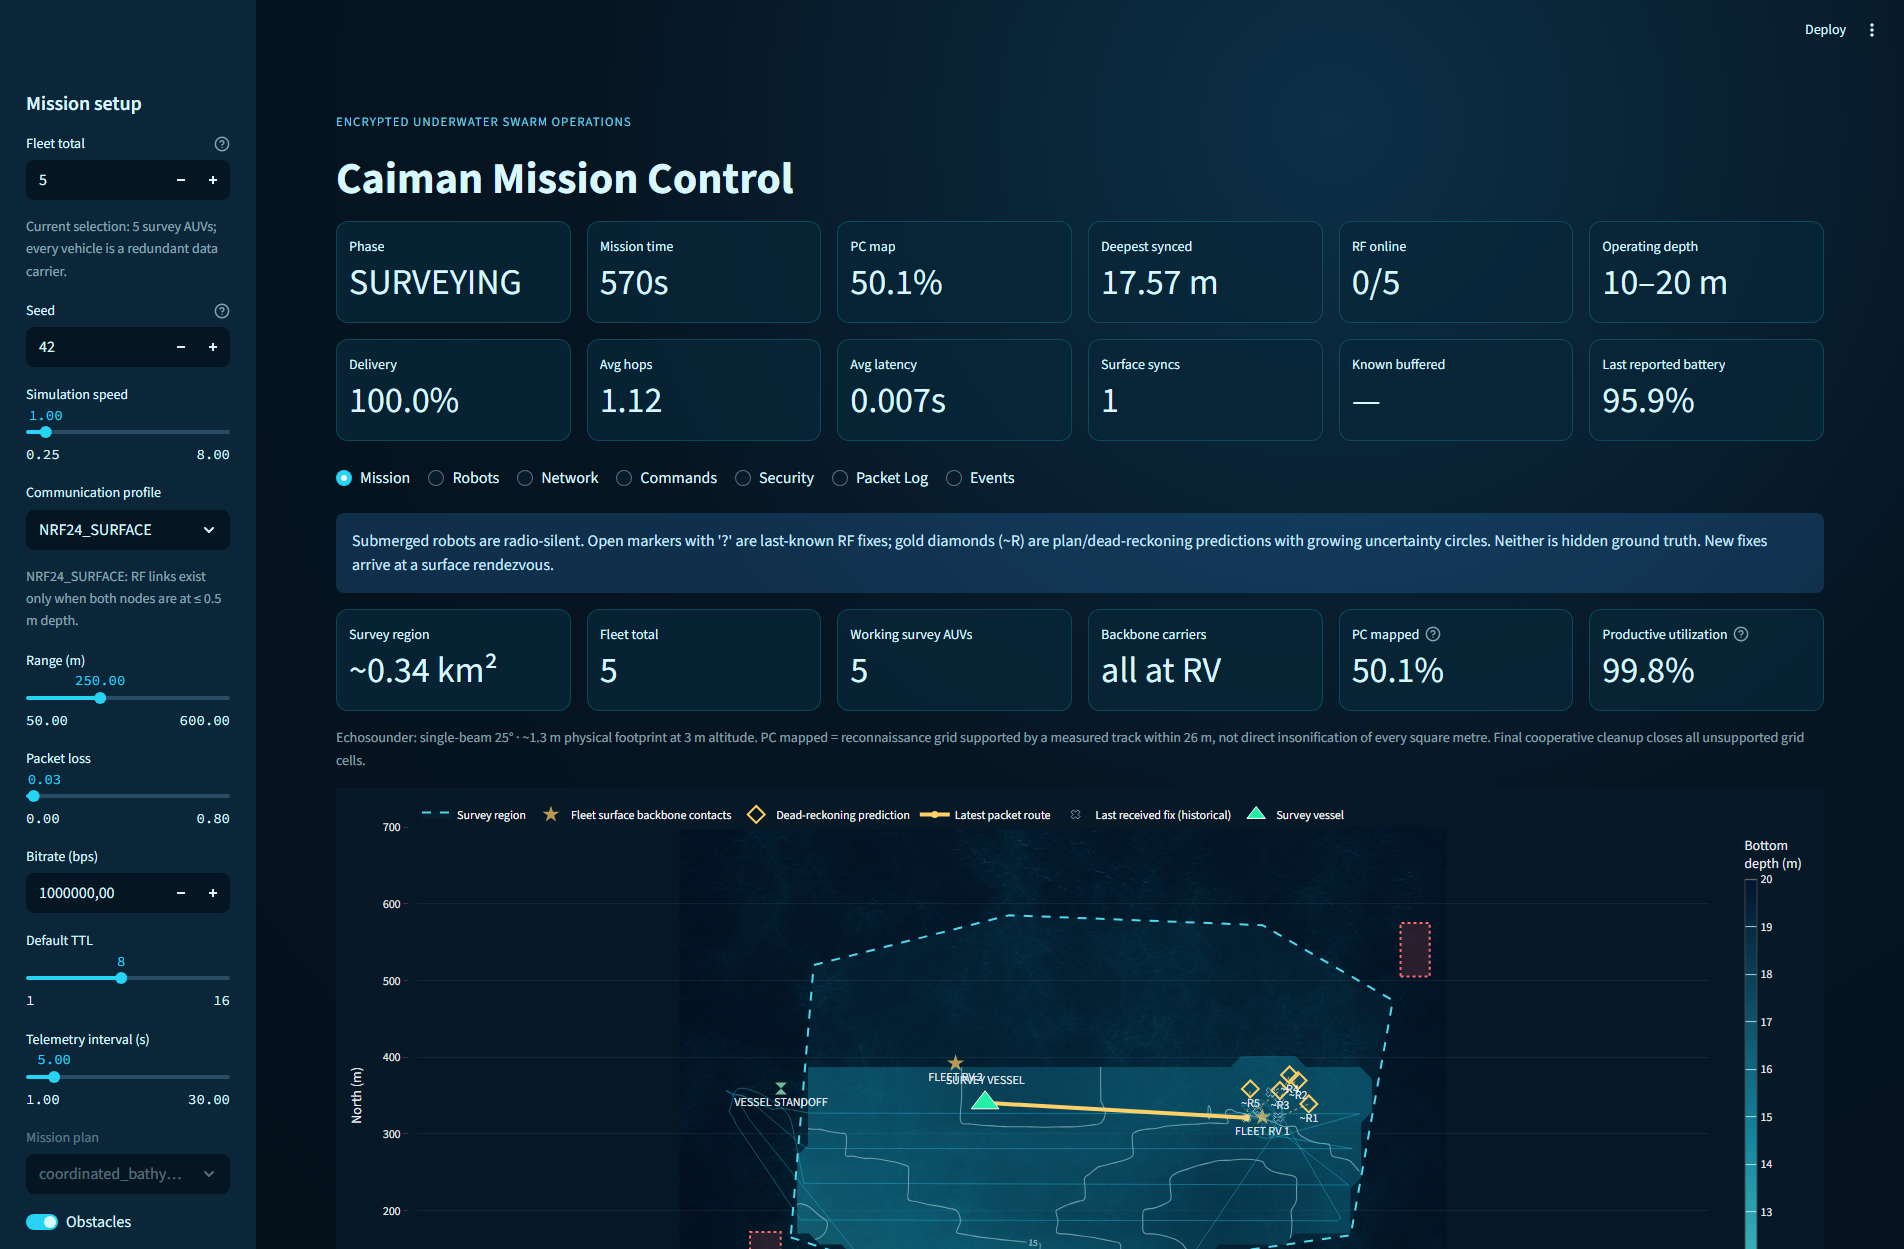
\includegraphics[width=\textwidth]{simulator/mission_after_first_sync.png}
  \caption{Interface Mission après le premier rendez-vous : 50,1\,\% de la carte de reconnaissance a été synchronisée, puis les cinq AUV sont redevenus radio-silencieux en immersion.}
  \label{fig:sim-mission-sync}
\end{figure}

\section{Communication de surface et connaissance du PC}

Le profil principal, \texttt{NRF24\_SURFACE}, interdit tout voisinage radio dès que l'un des deux n\oe{}uds se trouve à plus de \SI{0.5}{\metre} de profondeur. La portée nominale, le débit, les pertes, la latence de base, le TTL et la période de télémétrie restent réglables ; les valeurs par défaut sont respectivement \SI{250}{\metre}, \SI{1}{\mega\bit\per\second}, 3\,\%, \SI{5}{\milli\second}, 8 et \SI{5}{\second}. Les robots immergés stockent donc leurs mesures jusqu'au contact suivant.

Cette règle définit un graphe de communication variable dans le temps. En notant $z_i$ la profondeur positive vers le bas, $\mathbf{p}_i$ la position du n\oe{}ud $i$, $R$ la portée et $\mathcal{I}(t)$ les liens volontairement interrompus, son adjacence s'écrit simplement
\begin{equation}
  a_{ij}(t)=
  \begin{cases}
    1, & \substack{i,j\text{ actifs},\ z_i(t),z_j(t)\leq \SI{0.5}{\metre},\\
      \lVert\mathbf{p}_i(t)-\mathbf{p}_j(t)\rVert_2\leq R,\ (i,j)\notin\mathcal{I}(t)},\\[1ex]
    0, & \text{sinon.}
  \end{cases}
  \label{eq:surface-graph}
\end{equation}
Avec $R=\SI{250}{\metre}$ par défaut, le graphe disparaît pendant l'immersion puis se reconstruit lors des rendez-vous. Une transmission multi-sauts n'est possible que si ce graphe contient un chemin entre l'émetteur et la station de base ; cette lecture relie directement le simulateur aux architectes de réseaux tolérants aux interruptions et aux réseaux sous-marins contraints \cite{fall2003delay, akyildiz2005underwater}.

Une contrainte importante est la séparation entre la vérité interne du simulateur et ce que le navire peut connaître. Après la plongée, l'interface fige la dernière position reçue par radio et la marque comme \texttt{LAST KNOWN}. Une seconde marque propage seulement la route commandée avec une incertitude croissante ; elle n'expose jamais la position exacte cachée. Lorsque la télémétrie retardée arrive au rendez-vous, les échantillons horodatés reconstruisent la trajectoire réellement parcourue au lieu de dessiner un saut instantané artificiel.

À la surface, les AUV disponibles forment temporairement un backbone redondant. Un flooding contrôlé transmet chaque couple source--séquence une seule fois, applique la portée et les pertes, limite les boucles par TTL et permet à un robot hors portée directe d'atteindre la station par plusieurs sauts. Les ACK et retransmissions sont journalisés séparément des paquets applicatifs.

\begin{figure}[htbp]
  \centering
  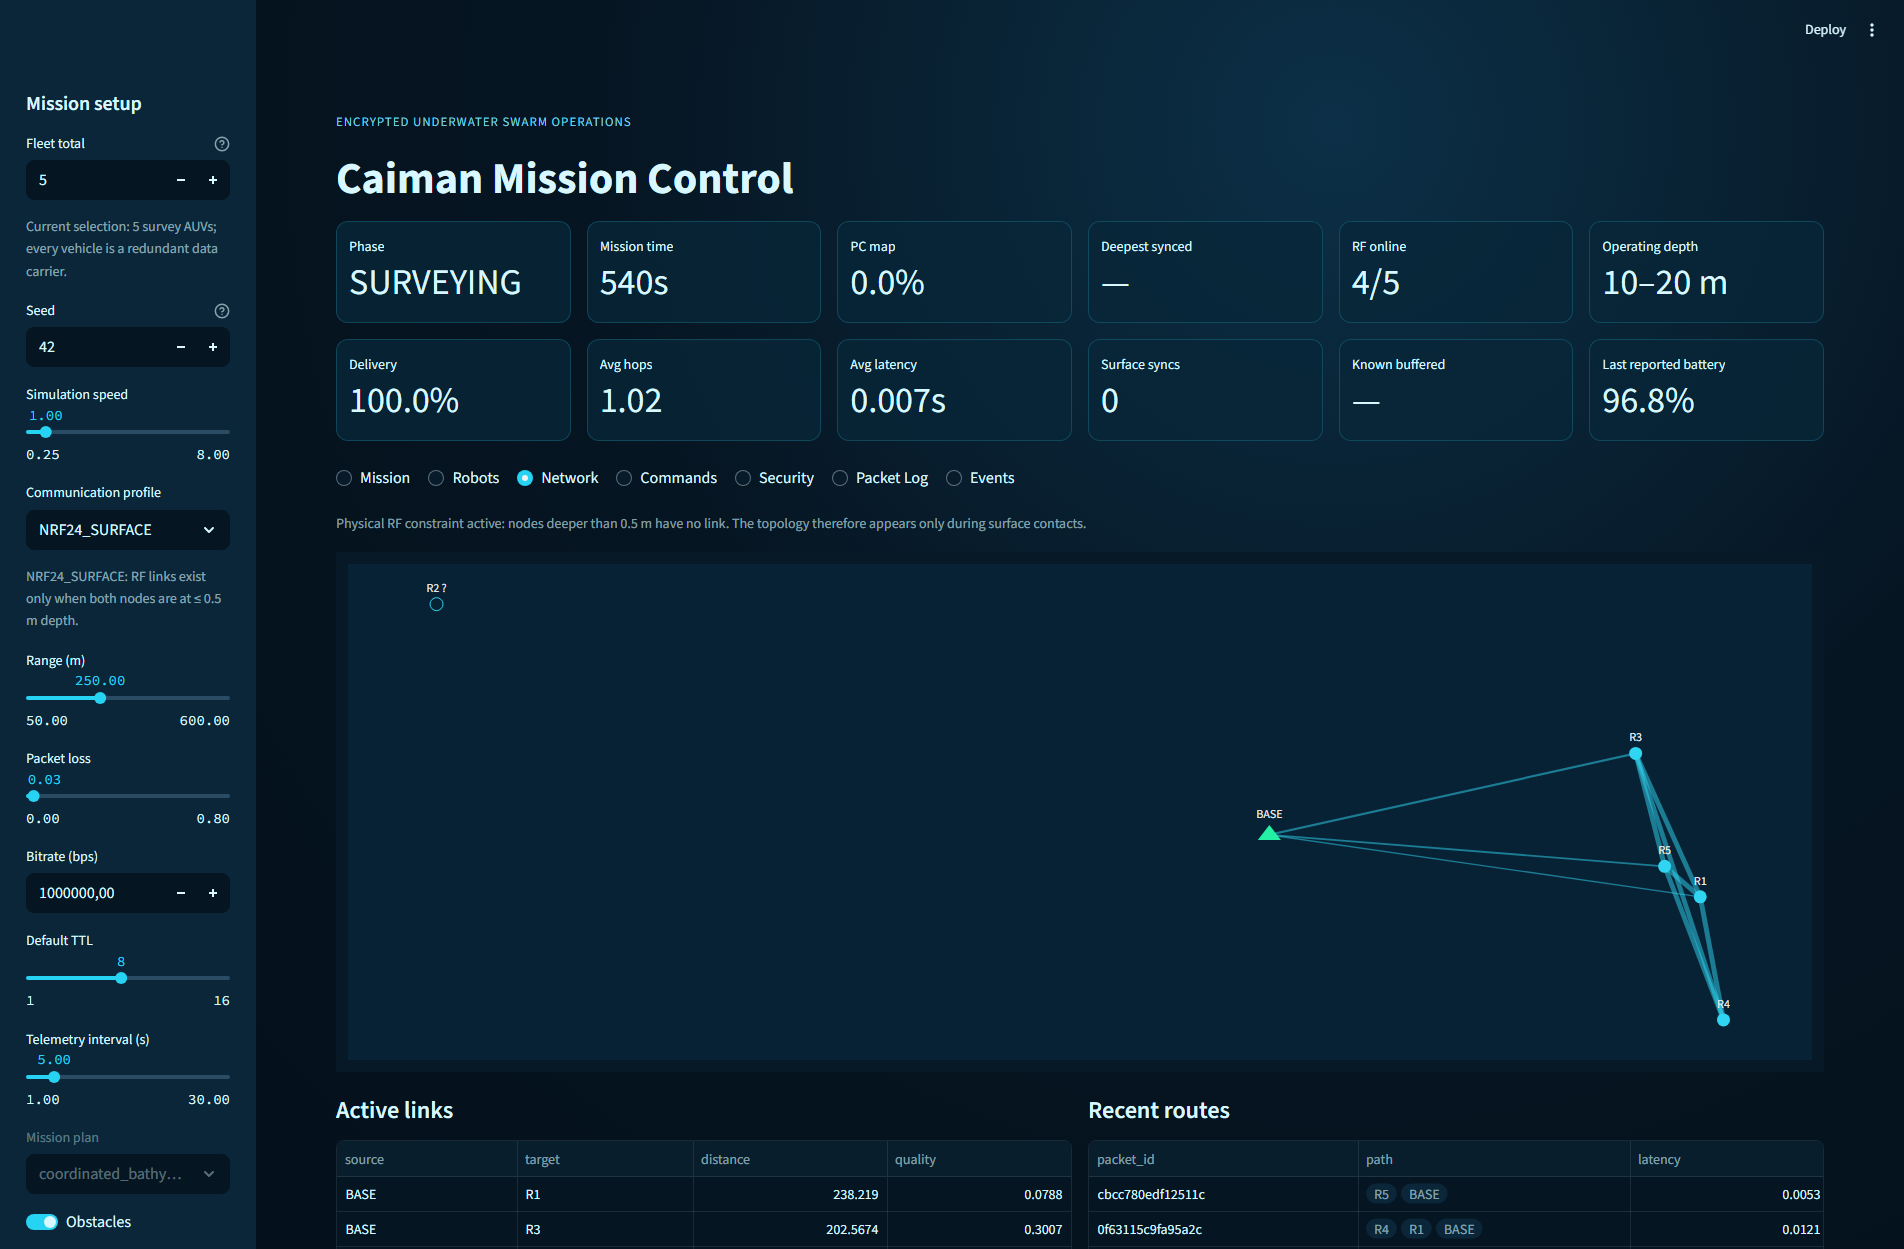
\includegraphics[width=\textwidth]{simulator/surface_mesh_rendezvous.png}
  \caption{Vue Network pendant un rendez-vous : quatre AUV sont déjà en surface, les liens actifs et une route multi-sauts vers la base sont visibles.}
  \label{fig:sim-network-mesh}
\end{figure}

\section{Trame compacte de 32 octets}

Le codec ne se contente pas de compter une taille logique : il génère des charges physiques de 32 octets, limite exacte du transcepteur nRF24 \cite{nordic-nrf24l01p}. Une télémétrie courante est compactée sur 64 bits : positions $x/y$, profondeur du véhicule et du fond, batterie, qualité de lien, fuite et disponibilité GNSS. La trame est répartie comme suit :

\begin{itemize}
  \item 8 octets d'en-tête : contrôle, source, destination, séquence, fragment et longueur utile ;
  \item 8 octets de charge chiffrée ;
  \item 16 octets pour l'étiquette Poly1305 complète.
\end{itemize}

Les messages plus longs utilisent au maximum seize fragments, chacun authentifié indépendamment. Les relais retransmettent les 32 octets immuables et conservent TTL et nombre de sauts dans leur politique locale ; ils ne réécrivent donc ni le texte chiffré ni son authentificateur.

La charge applicative occupe ainsi
\begin{equation}
  \eta_{\mathrm{app}}=\frac{8}{32}=25\,\%,
  \qquad
  N_{\mathrm{frag}}=\left\lceil\frac{B}{8}\right\rceil,
  \label{eq:frame-efficiency}
\end{equation}
où $B$ est la taille du message en octets. La limite de seize fragments porte donc la charge utile logique maximale à 128 octets. Les 75\,\% restants ne sont pas une perte arbitraire : ils portent l'adressage, le séquencement et surtout l'authentification. Il s'agit d'une efficacité de trame applicative, pas d'un rendement mesuré de la couche radio.

\begin{figure}[htbp]
  \centering
  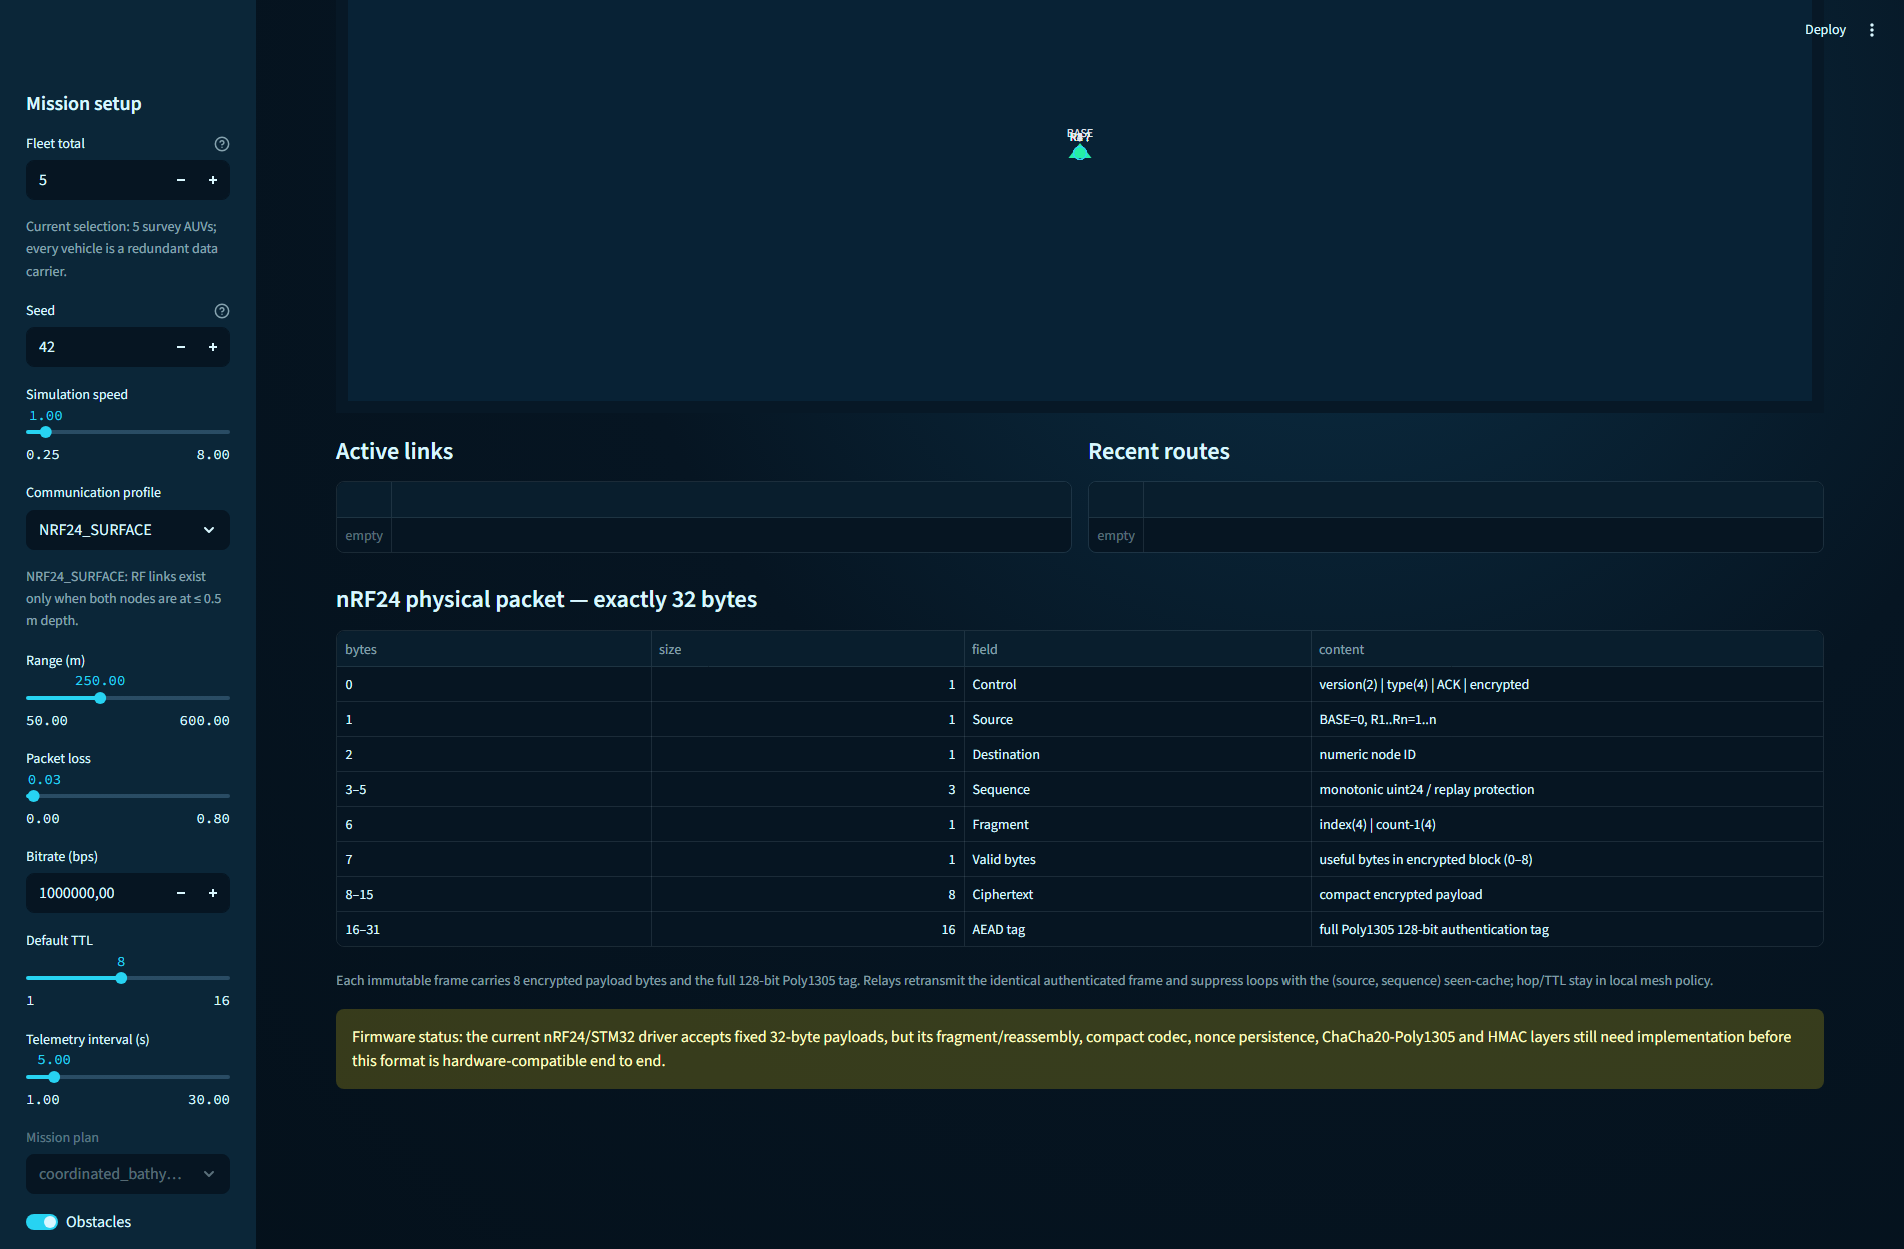
\includegraphics[width=\textwidth]{simulator/nrf24_frame_32_bytes.png}
  \caption{Décomposition octet par octet de la trame nRF24 chiffrée et authentifiée produite par le simulateur.}
  \label{fig:sim-frame32}
\end{figure}

Cette spécification est plus avancée que le chemin radio actuel du STM32 : le pilote sait transporter une charge fixe de 32 octets, mais la fragmentation, le codec compact, ChaCha20-Poly1305 et la persistance sûre du compteur de nonce restent à porter dans le firmware final.

\section{Sécurité et scénarios de défaut}

Chaque mission crée une clé maître aléatoire de 256 bits. HKDF-SHA-256 (RFC 5869 \cite{rfc5869}), dont le principe d'extraction puis d'expansion est établi par Krawczyk \cite{krawczyk2010hkdf}, en dérive des matériaux distincts pour le chiffrement, le routage et l'empreinte affichée. ChaCha20-Poly1305 (RFC 8439 \cite{rfc8439}) protège la confidentialité et l'authenticité du contenu. Ce choix repose sur la construction de flux de Bernstein \cite{bernstein2008chacha} et sur le modèle de chiffrement authentifié avec données associées formalisé par Rogaway \cite{rogaway2002authenticated} ; il convient à un microcontrôleur dépourvu d'accélérateur AES. Une séquence monotone par source et un préfixe de mission participent à la construction des nonces. Une fenêtre anti-rejeu rejette les anciennes séquences, tandis qu'un cache élimine les duplications de relais. L'interface n'affiche jamais la clé elle-même, seulement un identifiant et une empreinte tronquée.

La vue Security permet de modifier le texte chiffré, d'altérer l'étiquette AEAD, de corrompre l'authentification de route, de rejouer une ancienne trame et de provoquer une rotation de clé. Elle injecte également la mise hors ligne, une batterie critique, une fuite ou l'isolement réseau d'un robot. Les rejets sont comptés par catégorie afin de ne pas confondre perte de transport, doublon, rejeu et échec d'authentification.

Le scénario de capture physique relie sécurité et contraintes du milieu. Le robot choisi est déclaré capturé et sa clé compromise. Les autres AUV, encore immergés, ne reçoivent aucun rappel fictif : ils poursuivent jusqu'à leur prochain contact de surface, reçoivent alors l'ordre authentifié de retour, sont récupérés, puis reçoivent une nouvelle clé dont le n\oe{}ud capturé est exclu.

\begin{figure}[htbp]
  \centering
  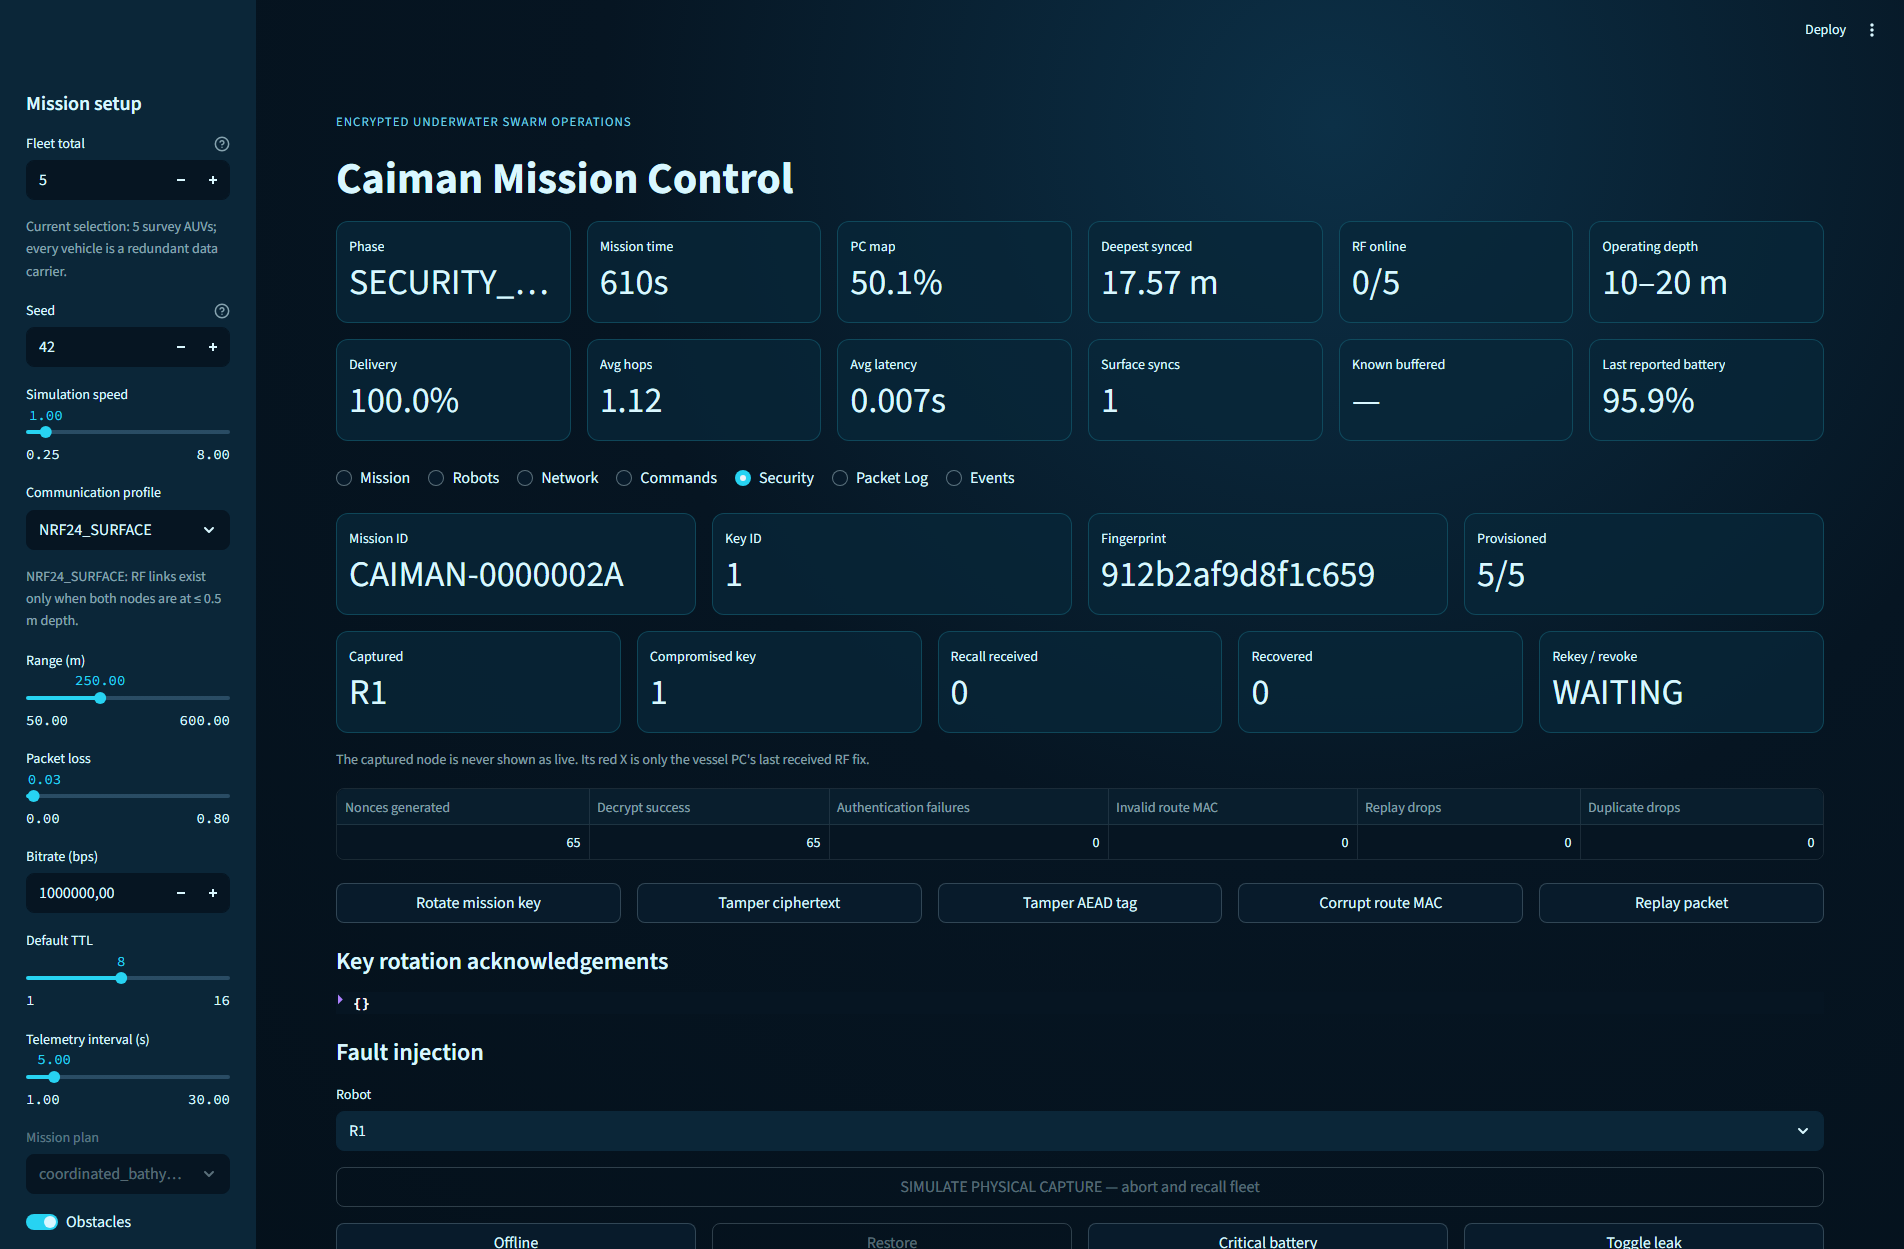
\includegraphics[width=\textwidth]{simulator/security_physical_capture.png}
  \caption{Début du scénario de capture de R1 : clé~1 compromise, rappel encore non reçu sous l'eau et renouvellement en attente.}
  \label{fig:sim-security-capture}
\end{figure}

Le choix actuel d'une clé de groupe simplifie la démonstration mais implique que la compromission d'un membre expose le groupe. Une évolution de production devra utiliser une racine propre à chaque véhicule, des clés de trafic par paire et une clé de routage de courte durée distribuée aux seuls membres autorisés.

\section{Interface opérateur, tests et exports}

Le tableau de bord \emph{Caiman Mission Control} regroupe sept vues complémentaires, présentées dans le \cref{tab:sim-views}.

\begin{table}[htbp]
  \centering
  \caption{Fonctions des vues de supervision.}
  \label{tab:sim-views}
  \begin{tabularx}{\textwidth}{@{}l X@{}}
    \toprule
    \textbf{Vue} & \textbf{Informations et actions principales} \\
    \midrule
    Mission & Bathymétrie reçue, trajectoires synchronisées, dernières positions radio, estimations et route récente. \\
    Robots & Télémétrie effectivement reçue : âge du fix, profondeur, batterie, fuite et qualité de lien. \\
    Network & Topologie de surface, liens, routes, latences, trame hexadécimale et disposition des 32 octets. \\
    Commands & Composition des ordres et suivi des ACK, délais et retransmissions. \\
    Security & Identité de clé, compteurs, attaques, capture, rotation et défauts. \\
    Packet Log & Journal filtrable du routage et de la livraison des paquets. \\
    Events & Chronologie unifiée de mission, réseau, commande, sécurité et défauts. \\
    \bottomrule
  \end{tabularx}
\end{table}

La suite automatique actuelle contient 33 tests : 2 pour le codec compact, 5 pour la cryptographie, 5 pour le réseau, 1 pour l'immuabilité au relais, 2 pour l'anti-rejeu et 18 pour la simulation complète. Elle vérifie notamment le déterminisme, la cohérence des capteurs virtuels, la batterie, l'absence de RF sous l'eau, les rendez-vous, le backbone des cinq AUV, les ACK, les retransmissions, les attaques, la rotation de clé et la capture. L'exécution de référence sur \GitCommit{77a253e} se termine par \texttt{33 passed}.

Le bouton d'export produit six fichiers horodatés : télémétrie CSV, paquets CSV, bathymétrie cartographiée CSV, mission complète JSON, configuration JSON et résumé JSON. Ces artefacts permettent une analyse hors ligne et rendent les paramètres d'une démonstration traçables.

\section{Déploiement Web}

Afin de rendre le démonstrateur utilisable sans installer Python, l'application a été conteneurisée puis déployée sur une VPS. Un conteneur Python~3.12 exécute Streamlit sur le port~8501 ; un second conteneur Caddy assure le proxy inverse, la compression et l'exposition HTTP/HTTPS. Un contrôle de santé interroge périodiquement \path{/_stcore/health}. Le domaine configuré est \url{https://caimansim.fr}, avec \url{https://www.caimansim.fr} comme alias.

L'hébergement s'appuie sur une souscription Azure ouverte au titre des crédits étudiants, ce qui conditionne la disponibilité publique à la validité de ces crédits. Le 16 août 2026, l'instance locale reconstruite à partir du dépôt répondait \texttt{200 ok} et a servi aux captures des \cref{fig:sim-mission-sync,fig:sim-network-mesh,fig:sim-frame32,fig:sim-security-capture} ; le DNS public résolvait toujours vers la machine, mais les ports HTTP/HTTPS ne répondaient plus depuis le poste d'audit, l'instance ayant vraisemblablement été suspendue à l'épuisement des crédits. Ce qui est démontré ici est donc la chaîne de déploiement --- conteneurisation, proxy inverse, contrôle de santé, nom de domaine --- et non une disponibilité continue, qui dépend d'un hébergement pérenne restant à financer.

\section{Limites du modèle}

Le terrain reste synthétique, la cinématique ne modélise ni hydrodynamique ni collision détaillée et le passage air--eau de l'antenne est ramené à un seuil binaire. Les profils acoustiques décrivent délais et pertes, pas les formes d'onde ni le DSP d'un modem. Le flooding n'inclut pas la contention du médium et le modèle énergétique ne constitue pas une mesure d'autonomie. Enfin, GNSS et Ping2 restent des données virtuelles tant que leurs pilotes matériels ne sont pas intégrés. Ces limites définissent précisément le passage nécessaire vers le HIL puis vers le PCB final.

\section{Prototype HIL}

Le commit \GitCommit{77a253e} ajoute une implémentation C portable du protocole, une cible ESP32, une cible Raspberry Pi et un modèle du comportement nRF24. Conformément aux principes de la simulation matérielle dans la boucle (Hardware-in-the-Loop, HIL) \cite{monti2017hil}, la version de travail déployée sur le banc organise en outre un scénario bidirectionnel \texttt{node\_node} : l'ESP32 représente le robot R1 et le Raspberry Pi le robot R2. Les deux processeurs sont physiques ; le transport entre eux utilise le Wi-Fi et UDP, tandis que les contraintes principales du nRF24 sont reproduites par logiciel. Cet essai ne valide donc ni l'interface SPI ni les performances radio réelles du nRF24.

Le 16 août 2026, le firmware a été compilé avec ESP-IDF~6.0.2 puis écrit sur un ESP32-D0WDQ6 par l'interface série CP210x. Le second n{\oe}ud est un Raspberry Pi~4 Model~B Rev.~1.5. Le Raspberry s'est connecté au point d'accès \texttt{CAIMAN-HIL} créé par l'ESP32 ; les adresses utilisées étaient respectivement \texttt{192.168.4.2} et \texttt{192.168.4.1}.

Avant l'essai matériel, les deux exécutables natifs ont été recompilés sur le Raspberry avec GCC~14.2.0, CMake~3.31.6 et Mbed TLS~3.6.5. Les deux tests C ont réussi : codec, chiffrement authentifié, altération et anti-rejeu d'une part ; FIFO, interruptions, retransmissions et doublons du modèle nRF24 d'autre part.

La démonstration a ensuite demandé cinq échanges complets R1--R2--R1. Les cinq trames émises par R1 ont été authentifiées et décodées par R2, puis les cinq réponses de R2 ont été authentifiées et décodées par R1. Chaque message conservait une longueur de 32 octets et une charge utile chiffrée/authentifiée, et les numéros de séquence restaient monotones de part et d'autre.

Le banc a été exécuté deux fois dans la journée du 16 août 2026, à partir du même binaire et du même matériel. La première exécution, consignée dans un journal de synthèse, porte les séquences 102416 à 102420 pour R1 et 24577 à 24581 pour R2 ; trois réponses de R2 y ont demandé une retransmission simulée avant \texttt{TX\_DS}, et un \texttt{MAX\_RT} initial sur la séquence 102415 a été observé avant le démarrage du récepteur, hors des cinq cycles demandés. La seconde exécution a fait l'objet d'une capture directe des deux terminaux ; c'est elle qui est reproduite au \cref{chap:validation}, avec des compteurs de séquence propres à cette exécution. Les deux journaux sont conservés dans le dépôt.

Le résultat établit le fonctionnement du protocole portable, de la sécurité et de l'ordonnancement bidirectionnel sur deux processeurs réels. Il reste limité par le remplacement du support nRF24 par un modèle logiciel transporté sur Wi-Fi/UDP et par l'absence de la carte Caiman finale.

\begin{figure}[htbp]
  \centering
  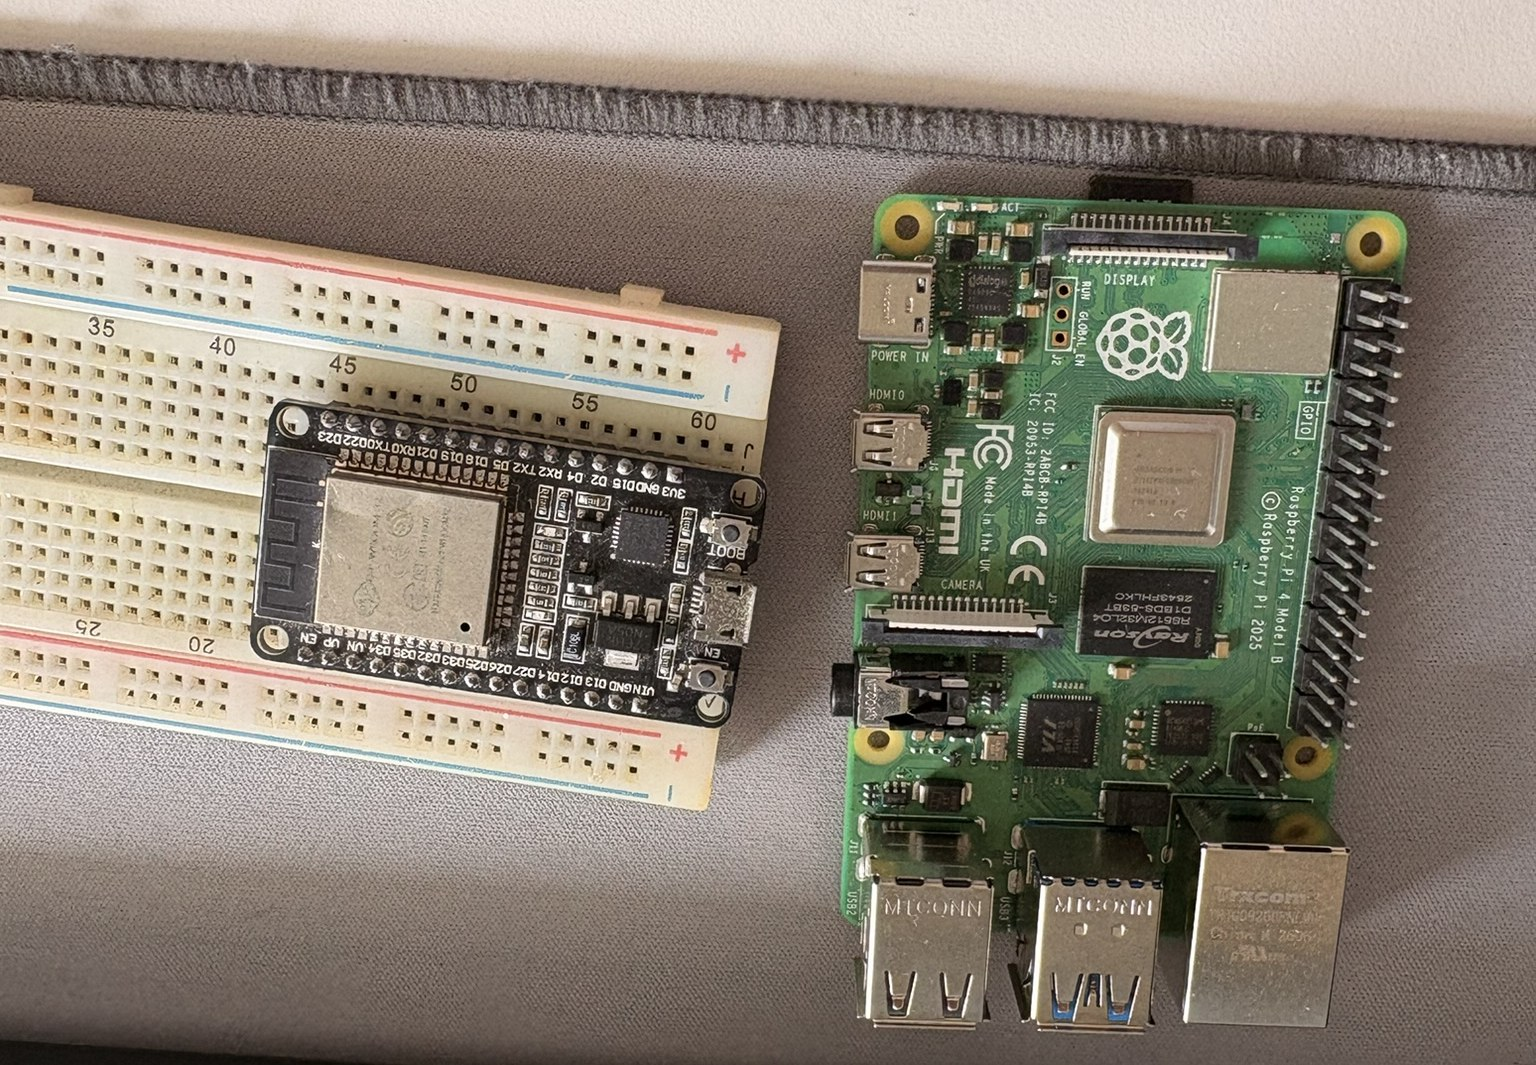
\includegraphics[width=0.85\textwidth]{hil/hil_banc_2026-08-16.jpg}
  \caption{Matériel du banc HIL le 16 août 2026 : à gauche la carte de développement ESP32 sur plaque d'essai, tenant le rôle du robot R1 ; à droite le Raspberry Pi~4 Model~B, tenant celui de R2. La photographie documente les deux n\oe{}uds physiques ; la preuve de l'exécution est fournie par les journaux du banc.}
  \label{fig:hil-setup}
\end{figure}

\chapter{Stratégie de validation et résultats}
\label{chap:validation}

La validation est organisée selon cinq niveaux afin de ne pas confondre présence de code, prototype de développement et fonctionnement du système final.

\begin{enumerate}
  \item \emph{CAO électronique} : contrôles ERC et DRC reproductibles, inspection du schéma, du routage, de la BOM et des fichiers de production, complétés par la revue DFM du fabricant (\cref{sec:drc}).
  \item \emph{Logiciel de simulation} : 32 tests Python passent sur l'état \GitCommit{4162c87} et 33 sur \GitCommit{77a253e}.
  \item \emph{Prototype STM32/IMU} : essai exploratoire documenté par photographies, sans mesure métrologique ni validation du matériel final.
  \item \emph{Prototype de protocole} : compilation et tests C sur Raspberry Pi, flash de l'ESP32 et cinq échanges HIL bidirectionnels authentifiés.
  \item \emph{PCB final} : aucun test physique, faute de réception avant la date de remise.
\end{enumerate}

\section{Résultats reproductibles}

Le \cref{tab:validation} associe à chaque résultat annoncé le niveau de preuve effectivement disponible.

\begin{table}[H]
  \centering
  \caption{Synthèse du niveau de preuve obtenu.}
  \label{tab:validation}
  \begin{tabularx}{\textwidth}{@{}X l X@{}}
    \toprule
    \textbf{Résultat} & \textbf{État} & \textbf{Preuve} \\
    \midrule
    Zéro erreur ERC bloquante & démontré & KiCad 10.0.5 ; 42 avertissements subsistent. \\
    Zéro élément PCB non connecté & démontré & DRC de \GitCommit{b58eda6}. \\
    DRC sans violation bloquante & démontré & 1 clearance résiduelle à \SI{0.1291}{\milli\metre} sur \GitCommit{b58eda6}, au-dessus de la capacité du procédé et documentée en exclusion (\cref{sec:drc}). \\
    Tests Python du simulateur & démontré & 32/32 sur \GitCommit{4162c87} ; 33/33 sur \GitCommit{77a253e}. \\
    Banc STM32/ICM-20948 & documenté & NUCLEO-H743ZI2 et module neuf axes photographiés ; résultats seulement qualitatifs. \\
    Tests C natifs du protocole & démontré & 2/2 tests réussis sur Raspberry Pi~4, GCC~14.2.0 et Mbed TLS~3.6.5. \\
    HIL ESP32--Raspberry Pi & démontré & 5/5 cycles bidirectionnels R1--R2--R1 ; trames de 32 octets authentifiées et séquences monotones. \\
    Bring-up PCB Caiman & non réalisé & carte en attente de réception. \\
    \bottomrule
  \end{tabularx}
\end{table}

Cette synthèse permet ainsi de défendre le travail accompli sans transformer les limites calendaires en résultats techniques inexistants. Les deux sections suivantes détaillent le seul niveau où deux processeurs physiques ont été mis en jeu.

\section{Validation du banc Hardware-in-the-Loop (HIL) bidirectionnel}

Le banc HIL associe deux processeurs physiques : un microcontrôleur ESP32 (représentant l'AUV R1) et un nano-ordinateur Raspberry Pi 4 (représentant l'AUV R2 ou la station de surface). Ce banc valide la chaîne logicielle C embarquée (sérialisation des trames de 32 octets, chiffrement/authentification AEAD ChaCha20-Poly1305, dérivation de clés HKDF et contrôle d'anti-rejeu par numéro de séquence monotone).

Cinq cycles complets d'échange bidirectionnel (\emph{ping-pong} authentifié R1 $\rightarrow$ R2 $\rightarrow$ R1) ont été exécutés avec succès. Les journaux ci-dessous en constituent la trace directe.

Le matériel employé est celui décrit en \cref{fig:hil-setup}. Le \cref{tab:hil-cycles} résume les cinq cycles tels que relevés simultanément sur les deux terminaux : pour chacun, la trame émise par R1 est authentifiée et décodée par R2, qui répond par une trame elle-même authentifiée et décodée par R1, l'acquittement du modèle nRF24 étant confirmé par un \texttt{TX\_DS}.

\begin{table}[H]
  \centering
  \small
  \caption{Synthèse des cinq cycles bidirectionnels relevés le 16 août 2026 sur les deux n\oe{}uds physiques.}
  \label{tab:hil-cycles}
  \begin{tabular}{@{}ccccccc@{}}
    \toprule
    \textbf{Cycle} & \multicolumn{3}{c}{\textbf{R1 $\rightarrow$ R2}} & \multicolumn{3}{c}{\textbf{R2 $\rightarrow$ R1}} \\
    \cmidrule(lr){2-4}\cmidrule(lr){5-7}
    & séquence & auth. & \texttt{TX\_DS} & séquence & auth. & \texttt{TX\_DS} \\
    \midrule
    1 & 102762 & OK & OK & 32769 & OK & OK \\
    2 & 102763 & OK & OK & 32770 & OK & OK \\
    3 & 102764 & OK & OK & 32771 & OK & OK \\
    4 & 102765 & OK & OK & 32772 & OK & OK \\
    5 & 102766 & OK & OK & 32773 & OK & OK \\
    \bottomrule
  \end{tabular}
\end{table}

Les séquences sont strictement croissantes de part et d'autre, condition nécessaire au rejet des rejeux. Le \cref{lst:hil-extrait} en donne un cycle représentatif, tel que capturé sur le Raspberry Pi ; les journaux complets des deux n\oe{}uds figurent en \cref{app:evidence}.

\begin{lstlisting}[
  caption={Cycle 1 relevé sur le n\oe{}ud R2 (Raspberry Pi~4) : réception authentifiée, trame chiffrée de 32 octets, puis réponse acquittée.},
  label={lst:hil-extrait},
  basicstyle=\ttfamily\small,
  frame=single,
  breaklines=true
]
R2 RX PEER_STATE seq=102762 R1->R2 | x=123.9m y=456.9m depth=12.10m
   bottom=18.55m battery=79.5% link=0% leak=no GNSS=no
R2 FRAME 32B encrypted=41010201916a00083a07039bff1df48a...
R2 TX PEER_STATE seq=32769 R2->R1 x=800.0 y=200.0 depth=10.00
   battery=95.0 link=100%
R2 TX PEER_STATE seq=32769 -> TX_DS
\end{lstlisting}

Le journal de R1 se termine par une sixième émission sans destinataire (\texttt{seq=102767 -> MAX\_RT}) : le processus R2 avait été lancé avec \texttt{-{}-count 5} et s'était déjà arrêté. Cette ligne confirme au passage que la détection d'absence d'acquittement fonctionne, les cinq cycles utiles restant complets et acquittés.

\paragraph{Périmètre de validation matérielle.}
La frontière physique de cette validation se situe aux niveaux suivants :
\begin{itemize}
  \item L'ESP32 et le Raspberry Pi exécutent le code C natif de protocole réel.
  \item Le médium de transport physique intermédiaire utilisé sur ce banc de laboratoire est une liaison Wi-Fi/UDP simulant les paquets radio.
  \item Le comportement de la puce nRF24L01+ est modélisé de façon logicielle. Par conséquent, l'interface physique SPI et la propagation radio RF réelle avec les antennes sous-marines sur la carte Caiman restent non validées à ce stade.
\end{itemize}

\chapter{Gestion du projet et retour d'expérience}
\label{chap:gestion}

\section{Déroulement et planning}

Le stage s'étend du 1\textsuperscript{er} juin au 31 août 2026. Juin regroupe la prise en main expérimentale STM32/IMU, la correction du schéma et du PCB ainsi que la commande. Juillet est consacré au simulateur de flotte, à sa supervision Web, au scénario de capture et à son déploiement, puis au premier HIL. La reproduction physique du HIL, la rédaction et la préparation de la soutenance occupent le mois d'août. La \cref{fig:gantt} en donne la répartition.

\begin{figure}[htbp]
  \centering
  \begin{ganttchart}[
    hgrid,
    vgrid,
    x unit=2.65cm,
    title/.style={fill=enstablue!15},
    bar/.style={fill=caimanblue}
  ]{1}{3}
    \gantttitle{2026}{3} \\
    \gantttitle{Juin}{1}\gantttitle{Juillet}{1}\gantttitle{Août}{1} \\
    \ganttbar{Schéma et PCB}{1}{1} \\
    \ganttbar{Firmware}{1}{2} \\
    \ganttbar{Simulation}{2}{2} \\
    \ganttbar{HIL et rédaction}{2}{3}
  \end{ganttchart}
  \caption{Planning du stage reconstruit à partir de l'historique Git et des essais documentés.}
  \label{fig:gantt}
\end{figure}

\section{Difficultés rencontrées et inflexions du projet}

Trois écarts entre le plan initial et le déroulement réel méritent d'être exposés, moins pour eux-mêmes que pour les pratiques de travail qu'ils ont fait évoluer.

Le premier tient au délai de fabrication. La commande a été lancée le 23 juin, mais les délais cumulés de production et d'assemblage ne permettaient pas la réception avant la soutenance du \DefenseDate. La mission prévue par la convention --- fabriquer plusieurs robots puis les essayer en bassin --- devenait matériellement inatteignable. Plutôt que de laisser le projet en attente, la validation a été redirigée vers ce qui pouvait être éprouvé sans la carte : le protocole, son codage compact, sa sécurisation et son comportement en flotte. C'est de là que sont nés le simulateur puis le banc HIL. Cette réorientation ne contourne pas l'objectif, elle déplace le périmètre vérifiable ; elle impose en revanche de ne jamais présenter un résultat de simulation comme un résultat matériel, exigence qui a guidé la structuration du \cref{chap:validation}.

Le deuxième porte sur la sélection des composants. La revue PCBA du fabricant a détecté que les inductances de puissance présélectionnées, bien que de gabarit annoncé équivalent, présentaient des terminaisons débordant du \emph{land pattern} dessiné (\cref{sec:inductances}). Cette présélection reposait sur l'hypothèse implicite qu'un boîtier \enquote{$4\times4$\,mm} suffisait à caractériser un composant. La reprise a exigé de comparer, pour chaque candidat, la valeur d'inductance, le courant de saturation, la DCR et surtout la géométrie exacte des plages de brasage. La leçon est concrète : une nomenclature n'est pas une liste de valeurs, mais un ensemble d'engagements géométriques.

Le troisième est apparu lors d'un changement de poste de travail en cours de projet. Il a mis en évidence que tout ce qui conditionne la reproductibilité d'une commande --- règles de conception, liste d'exclusions DRC justifiées, dossier de production exporté, correspondance entre une révision et les fichiers réellement transmis --- doit être versionné au même titre que le schéma. Un fichier de production qui n'existe que sur un poste ne constitue pas une preuve. De là découle une règle de conduite retenue pour la suite. Le contrôle DRC doit être traité comme une condition de sortie de l'export de fabrication : réexécuté sur l'état exact qui alimente les fichiers transmis, puis archivé avec la commande. Il ne peut pas être considéré comme une étape franchie une fois pour toutes en cours de routage.

\section{Compétences mobilisées}

Le stage a mobilisé de manière transversale les disciplines clés du cursus d'ingénieur en robotique autonome. L'architecture des microcontrôleurs a été sollicitée par le firmware STM32, ses périphériques SPI/I\textsuperscript{2}C/UART et son ordonnancement FreeRTOS. La théorie du signal et de l'estimation intervient dans le filtrage complémentaire de l'\cref{eq:complementary-filter} et la modélisation du sonar de l'\cref{eq:sonar-footprint}. L'ingénierie des réseaux et de la communication contrainte apparaît enfin dans les trames de 32 octets, le routage distribué de l'\cref{eq:surface-graph} et la tolérance aux pannes. La démarche d'ingénierie système s'est appuyée sur les pratiques du génie logiciel : gestion de version, modularité du simulateur, journalisation et validation automatisée par tests unitaires et banc matériel.

Au-delà des techniques, l'apport principal de ce stage réside dans la qualification du statut des affirmations produites. Distinguer ce qui est conçu, implémenté, testé et validé ne relève pas de la précaution rhétorique : c'est la condition pour qu'un tiers sache sur quoi il peut s'appuyer. Cette exigence a façonné la structure même du présent rapport.

\chapter{Conclusion et perspectives}
\label{chap:conclusion}

Le stage a permis de faire évoluer une base électronique existante vers un dossier de fabrication, d'établir une première architecture firmware et de construire une chaîne progressive de validation. Après un banc exploratoire STM32/IMU, le simulateur de mission formalise le levé coopératif de cinq AUV, l'absence de radio sous l'eau, les rendez-vous de surface, la supervision, le protocole compact et les scénarios de sécurité. Sa conteneurisation et son déploiement Web en font également un démonstrateur autonome. Le HIL a ensuite exécuté cinq échanges bidirectionnels authentifiés entre un ESP32 et un Raspberry Pi réels, avec un modèle logiciel du lien nRF24.

Ce qui subsiste au-delà du stage ne se limite pas à un dossier de fabrication. Le simulateur, sa suite de tests et l'implémentation portable du protocole constituent des briques réutilisables par l'équipe : elles décrivent le comportement attendu d'une flotte Caiman indépendamment d'une carte particulière, et fournissent une référence contre laquelle le firmware définitif pourra être confronté. Le banc HIL, en exécutant ce même code C sur deux processeurs distincts, établit le pont entre cette référence et le monde physique ; il restera valable lorsque le transport Wi-Fi sera remplacé par le lien nRF24 réel.

La principale limite est l'absence de réception du PCB avant la rédaction. Aucun résultat de bring-up, de mesure d'alimentation, de capteur ou de radio sur la carte Caiman ne peut donc être revendiqué. La chaîne de vérification s'arrête à la CAO et à la revue de fabrication : elle établit que le dossier est cohérent et fabricable, non que la carte fonctionne.

Les prochaines étapes prioritaires en découlent directement : la réception et l'inspection visuelle des cartes, le contrôle de continuité des rails avant toute mise sous tension, la vérification des marges des inductances, la montée en tension avec limitation de courant, la mesure des rails, la programmation du STM32 puis le test progressif de chaque périphérique. L'intégration du protocole HIL au firmware de la carte permettra enfin de relier les résultats numériques au système physique.


\clearpage
\printbibliography[heading=bibintoc,title={Bibliographie}]

\clearpage
\chapter*{Glossaire français--anglais}
\addcontentsline{toc}{chapter}{Glossaire français--anglais}

\begin{longtable}{@{}>{\raggedright\arraybackslash}p{0.16\textwidth}>{\raggedright\arraybackslash}p{0.36\textwidth}>{\raggedright\arraybackslash}p{0.36\textwidth}@{}}
\toprule
\textbf{Sigle} & \textbf{Français} & \textbf{Anglais} \\
\midrule
\endhead
ACK & accusé de réception & acknowledgement \\
AEAD & chiffrement authentifié avec données associées & authenticated encryption with associated data \\
AUV & véhicule sous-marin autonome & autonomous underwater vehicle \\
BOM & nomenclature & bill of materials \\
CAO & conception assistée par ordinateur & computer-aided design \\
CPL & fichier de placement des composants & component placement list \\
DCR & résistance série en courant continu & DC resistance \\
DFM & conception orientée fabrication & design for manufacturability \\
DRC & contrôle des règles de conception & design rule check \\
ERC & contrôle des règles électriques & electrical rule check \\
GNSS & système mondial de navigation par satellite & global navigation satellite system \\
HIL & matériel dans la boucle & hardware-in-the-loop \\
HKDF & fonction de dérivation de clés fondée sur HMAC & HMAC-based key derivation function \\
IMU & centrale inertielle & inertial measurement unit \\
MCU & microcontrôleur & microcontroller unit \\
PCB & circuit imprimé & printed circuit board \\
PCBA & circuit imprimé assemblé & printed circuit board assembly \\
RF & radiofréquence & radio frequency \\
SPI & bus série synchrone à quatre fils & serial peripheral interface \\
UART & liaison série asynchrone & universal asynchronous receiver-transmitter \\
VPS & serveur privé virtuel & virtual private server \\
\bottomrule
\end{longtable}


\appendix
\chapter{Traçabilité et reproduction des résultats}
\label{app:evidence}

\section{Révisions de référence}

\begin{itemize}
  \item base amont : \GitCommit{5fc0681} ;
  \item révision PCB vérifiée au DRC : \GitCommit{b58eda6} ;
  \item état local et distant incluant la base du HIL : \GitCommit{77a253e} ;
  \item scénario HIL bidirectionnel : version de travail \texttt{node\_node} déployée sur le banc le 16 août 2026.
\end{itemize}

\section{Commandes principales}

\begin{lstlisting}[language=bash,caption={Simulateur de mission : installation, exécution et suite de tests.}]
cd simulator
python -m pip install -r requirements.txt
streamlit run app.py          # tableau de bord sur http://localhost:8501
python -m pytest tests -q     # suite de tests unitaires
\end{lstlisting}

\begin{lstlisting}[language=bash,caption={Contrôle DRC de la carte, exporté en JSON.}]
kicad-cli pcb drc --format json --units mm --severity-error \
  --severity-warning --output caiman_drc.json <chemin>/caiman.kicad_pcb
\end{lstlisting}

\begin{lstlisting}[language=bash,caption={Banc HIL : compilation native, flash de l'ESP32 et exécution bidirectionnelle.}]
cd /home/rasp/Caiman/protocol_hil
cmake -S . -B build && cmake --build build --parallel 4
ctest --test-dir build --output-on-failure

source /home/rasp/esp-idf-v6.0.2/export.sh
cd scenarios/node_node/esp32 && idf.py build
idf.py -p /dev/ttyUSB0 flash
sudo nmcli connection up caiman-hil ifname wlan0
cd /home/rasp/Caiman/protocol_hil
./build/caiman_node_r2 192.168.4.1 4210 --count 5
\end{lstlisting}

Le journal synthétique de l'essai est conservé dans
\path{rapport_stage/evidence/hil_2026-08-16.log}. Les deux tests natifs ont
réussi et le programme HIL s'est terminé avec un code de retour nul après cinq
cycles bidirectionnels.

\section{Journaux complets du banc HIL}

Les deux journaux ci-dessous ont été capturés simultanément le 16 août 2026 lors de la seconde exécution du banc. Le \cref{tab:hil-cycles} en donne la synthèse.

\begin{lstlisting}[
  caption={Sortie complète de \texttt{caiman\_node\_r2 192.168.4.1 4210 -{}-count 5} sur le Raspberry Pi~4.},
  label={lst:hil-r2},
  basicstyle=\ttfamily\scriptsize, frame=single, breaklines=true]
R2 node=2 listening on UDP 4210; peer R1=192.168.4.1 node=1

R2 RX PEER_STATE seq=102762 R1->R2 | x=123.9m y=456.9m depth=12.10m
   bottom=18.55m battery=79.5% link=0% leak=no GNSS=no
R2 FRAME 32B encrypted=41010201916a00083a07039bff1df48a...
R2 TX PEER_STATE seq=32769 R2->R1 x=800.0 y=200.0 depth=10.00
   battery=95.0 link=100%
R2 TX PEER_STATE seq=32769 -> TX_DS

R2 RX PEER_STATE seq=102763 R1->R2 | x=124.4m y=457.1m depth=12.20m
   bottom=18.60m battery=79.0% link=53% leak=no GNSS=no
R2 TX PEER_STATE seq=32770 R2->R1 x=799.7 y=200.4 depth=10.08
   battery=94.5 link=75%
R2 TX PEER_STATE seq=32770 -> TX_DS

R2 RX PEER_STATE seq=102764 R1->R2 | x=124.9m y=457.3m depth=12.30m
   bottom=18.65m battery=78.5% link=100% leak=no GNSS=no
R2 TX PEER_STATE seq=32771 R2->R1 x=799.4 y=200.8 depth=10.16
   battery=94.0 link=75%
R2 TX PEER_STATE seq=32771 -> TX_DS

R2 RX PEER_STATE seq=102765 R1->R2 | x=125.4m y=457.5m depth=12.40m
   bottom=18.70m battery=78.0% link=100% leak=no GNSS=no
R2 TX PEER_STATE seq=32772 R2->R1 x=799.1 y=201.2 depth=10.24
   battery=93.5 link=75%
R2 TX PEER_STATE seq=32772 -> TX_DS

R2 RX PEER_STATE seq=102766 R1->R2 | x=125.9m y=457.7m depth=12.50m
   bottom=18.50m battery=77.5% link=100% leak=no GNSS=no
R2 TX PEER_STATE seq=32773 R2->R1 x=798.8 y=201.6 depth=10.32
   battery=93.0 link=75%
R2 TX PEER_STATE seq=32773 -> TX_DS
\end{lstlisting}

\begin{lstlisting}[
  caption={Événements de diagnostic de l'ESP32 (R1), capturés par \texttt{caiman\_esp\_log 4211}.},
  label={lst:hil-r1},
  basicstyle=\ttfamily\scriptsize, frame=single, breaklines=true]
ESP32 HIL diagnostic events on UDP 4211
R1 TX PEER_STATE seq=102762 payload=8B frame=32B -> TX_DS
R1 RX PEER_STATE seq=32769 R2->R1 x=800.0 y=200.0 depth=10.00
   battery=95.0 link=100%
R1 TX PEER_STATE seq=102763 payload=8B frame=32B -> TX_DS
R1 RX PEER_STATE seq=32770 R2->R1 x=799.7 y=200.4 depth=10.08
   battery=94.5 link=73%
R1 TX PEER_STATE seq=102764 payload=8B frame=32B -> TX_DS
R1 RX PEER_STATE seq=32771 R2->R1 x=799.4 y=200.8 depth=10.16
   battery=94.0 link=73%
R1 TX PEER_STATE seq=102765 payload=8B frame=32B -> TX_DS
R1 RX PEER_STATE seq=32772 R2->R1 x=799.1 y=201.2 depth=10.24
   battery=93.5 link=73%
R1 TX PEER_STATE seq=102766 payload=8B frame=32B -> TX_DS
R1 RX PEER_STATE seq=32773 R2->R1 x=798.8 y=201.6 depth=10.32
   battery=93.0 link=73%
R1 TX PEER_STATE seq=102767 frame=32B -> MAX_RT
\end{lstlisting}

\section{Schéma électronique complet}

Le \cref{fig:schematic-annexe} reproduit le schéma KiCad complet dans une taille exploitable. Les extraits fonctionnels discutés dans le corps du rapport en sont issus.

\begin{figure}[htbp]
  \centering
  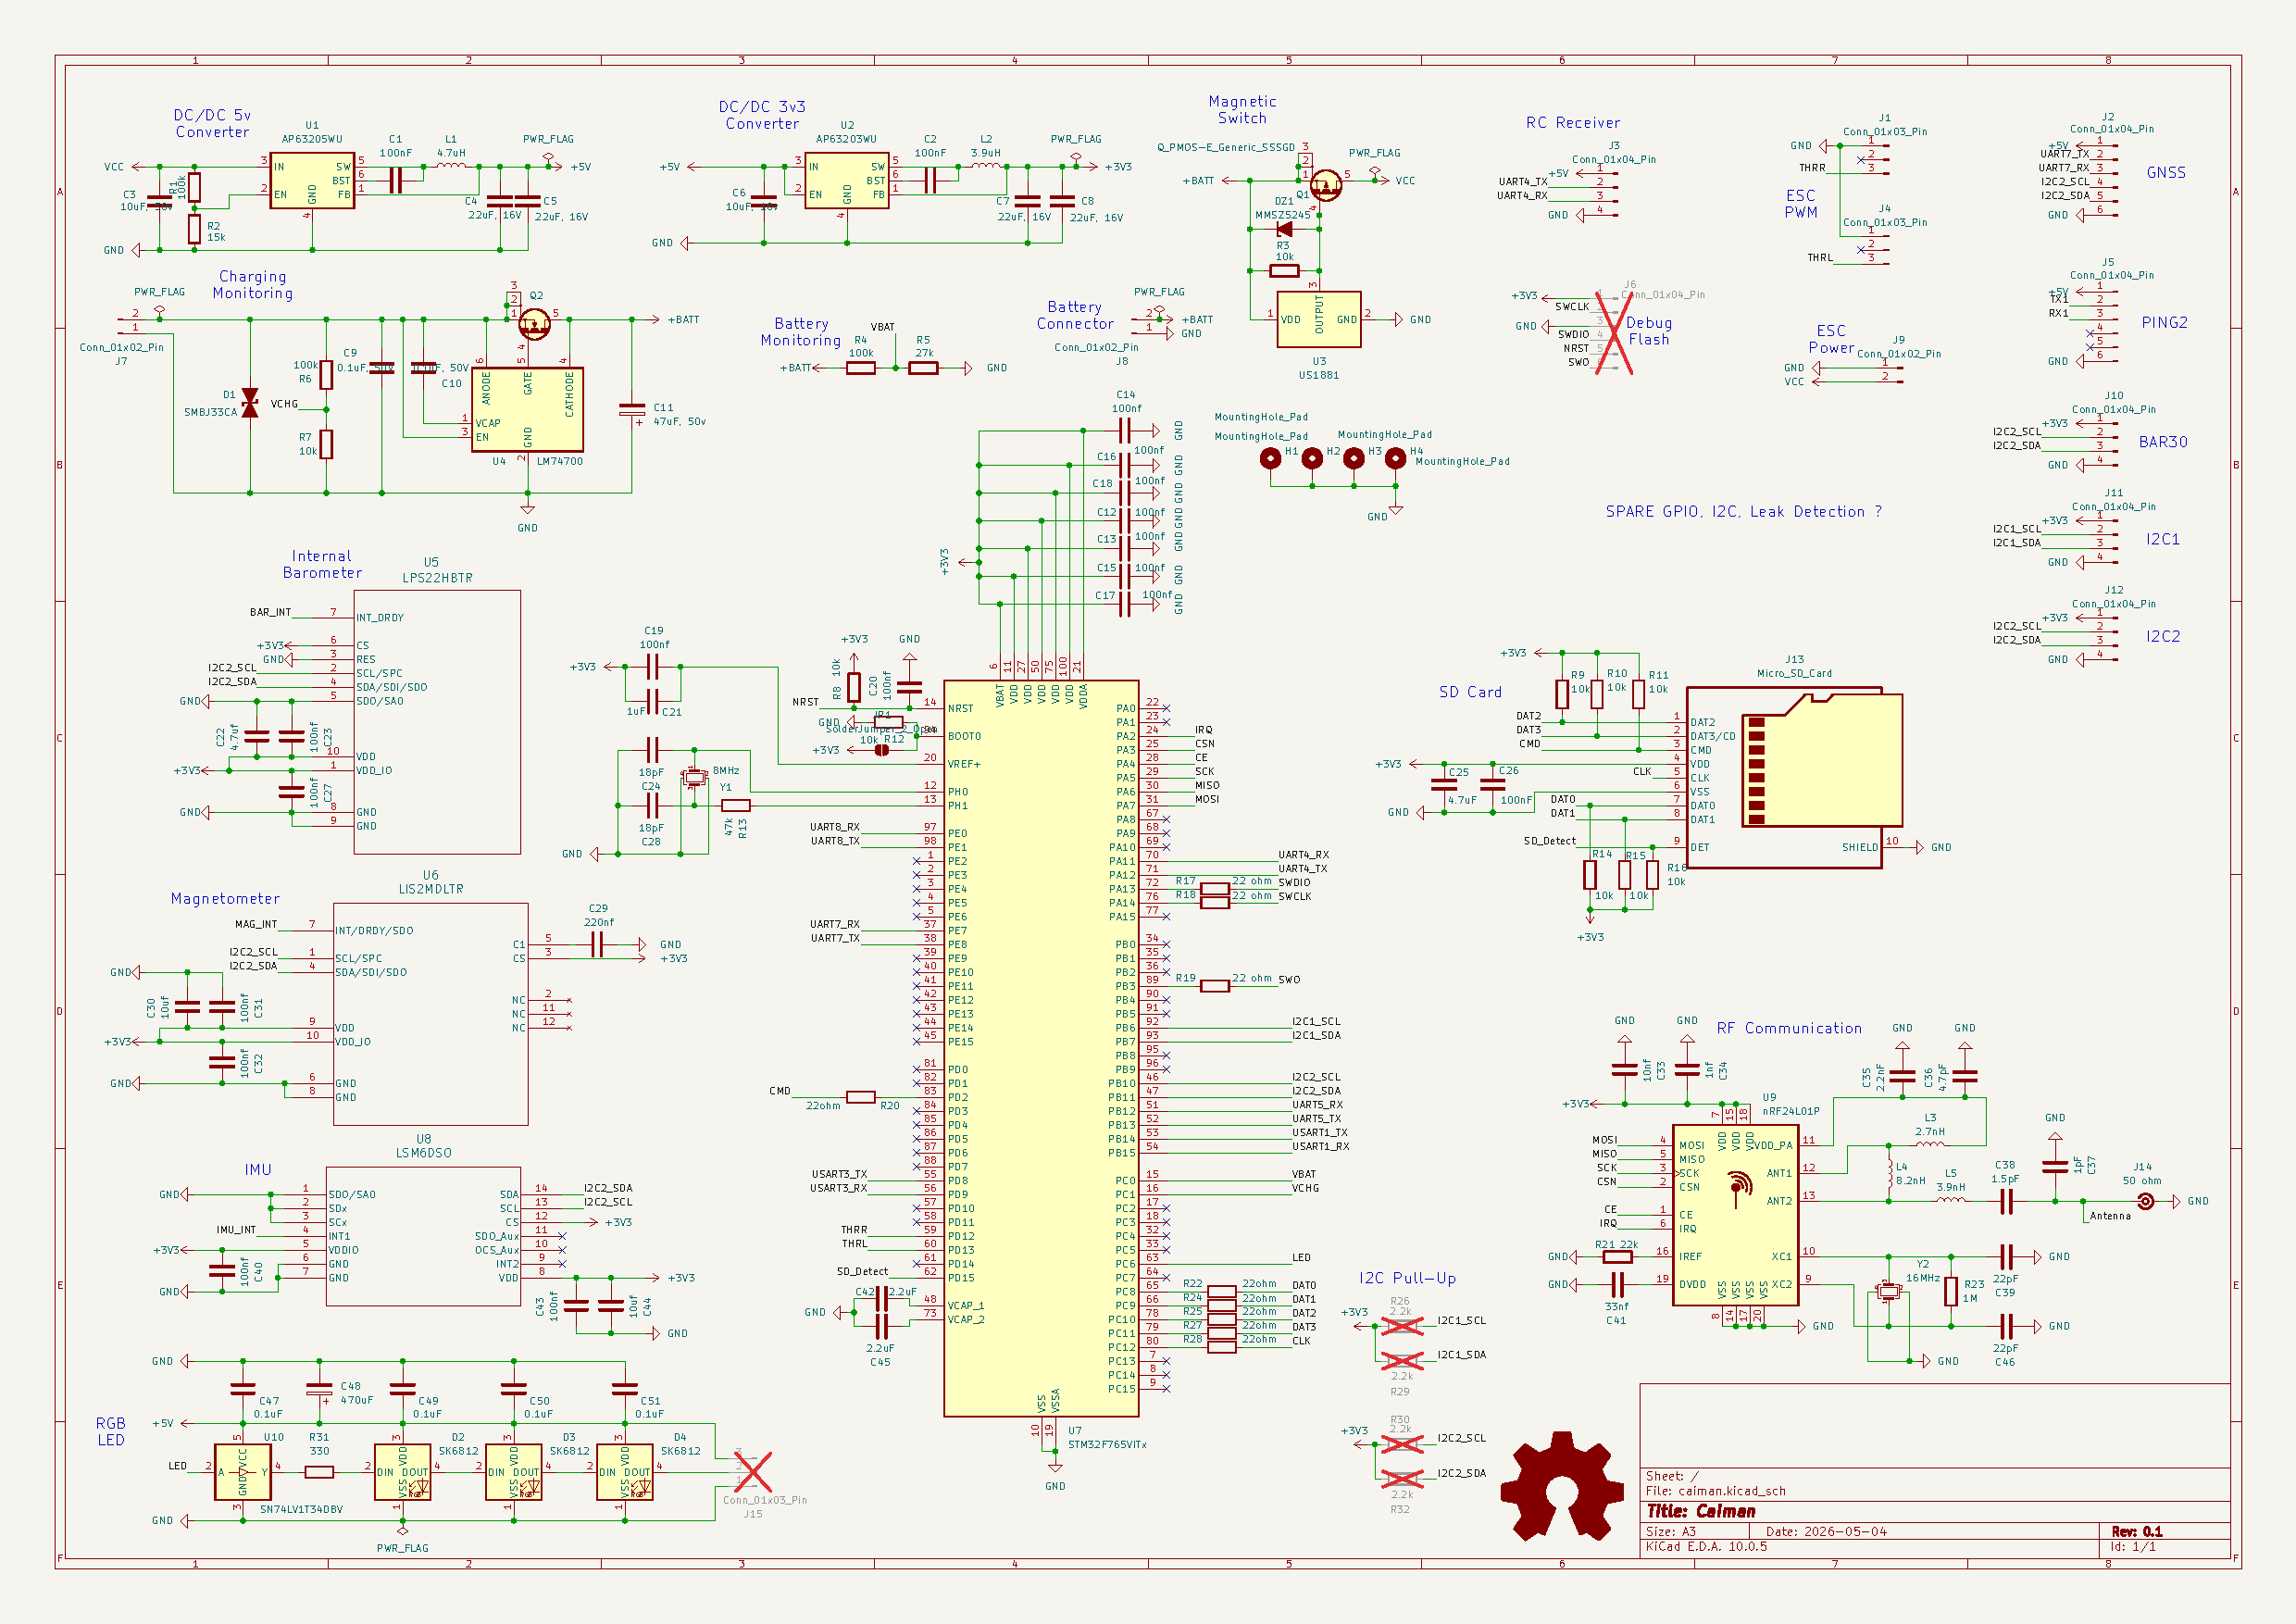
\includegraphics[width=\textwidth,height=0.82\textheight,keepaspectratio]{fabrication/caiman_schematic.pdf}
  \caption{Schéma électronique complet de la carte Caiman (microcontrôleur, alimentations, bus d'interfaçage et capteurs).}
  \label{fig:schematic-annexe}
\end{figure}

\section{Preuves complémentaires attendues}
\label{app:preuves}

\begin{itemize}\setlength{\itemsep}{0pt}
  \item journal ou tracé des lectures du banc STM32/ICM-20948 ;
  \item capture datée de \url{https://caimansim.fr} après remise en ligne ;
  \item photographies et relevés de continuité de la carte après réception ;
  \item résultats du bring-up, postérieurs à la soutenance si nécessaire.
\end{itemize}


\end{document}
